\documentclass[aspectratio=169]{beamer}

\usepackage{xcolor}
\usepackage{tikz}
\usepackage{stackrel}
\usepackage{bm,bbm}% bold math
\usepackage[version=3]{mhchem}
\usepackage{lmodern}

\usepackage{multirow}
\usepackage{setspace}
\usepackage{yfonts}
\usepackage{mathrsfs}
\usepackage{tcolorbox}
\usepackage{colortbl}
\usepackage{commath}
\usepackage{empheq}
\usepackage{multicol}
\usepackage{mhchem}
\usepackage[normalem]{ulem}
\usepackage{pifont}
\usepackage{fontawesome}
\usepackage{listings}

% Support for Pandoc-beamer
\usepackage[T1]{fontenc}
\usepackage{booktabs}
\usepackage{longtable}
\usepackage{fancyvrb}
\providecommand{\tightlist}{%
  \setlength{\itemsep}{0pt}\setlength{\parskip}{0pt}}

\usepackage[retainorgcmds]{IEEEtrantools}
\usepackage{siunitx}
\sisetup{detect-display-math=true,detect-weight=true,detect-family=true}

\usepackage{tcolorbox,xcolor,framed}
\DefineVerbatimEnvironment{Highlighting}{Verbatim}{fontsize=\footnotesize,commandchars=\\\{\}}
\definecolor{shadecolor}{rgb}{0.9,0.9,0.9}
\newenvironment{Shaded}{\snugshade}{\endsnugshade}
\newcommand{\KeywordTok}[1]{\textcolor[rgb]{0.13,0.29,0.53}{\textbf{#1}}}
\newcommand{\DataTypeTok}[1]{\textcolor[rgb]{0.13,0.29,0.53}{#1}}
\newcommand{\NormalTok}[1]{#1}
\newcommand{\DecValTok}[1]{\textcolor[rgb]{0.00,0.00,0.81}{#1}}
\newcommand{\CommentTok}[1]{\textcolor[rgb]{0.56,0.35,0.01}{\textit{{#1}}}}
\newcommand{\PreprocessorTok}[1]{\textcolor[rgb]{0.56,0.35,0.01}{\textit{{#1}}}}
\newcommand{\ControlFlowTok}[1]{\textcolor[rgb]{0.13,0.29,0.53}{\textbf{{#1}}}}


\usepackage[colorinlistoftodos, color=blue!20!white, bordercolor=gray,
textsize=tiny]{todonotes}

\setbeamercolor{structure}{fg=myOrange}
\setbeamercolor{normal text}{fg=myBlue}

\makeatletter
\newcommand*{\overlaynumber}{\number\beamer@slideinframe}
\makeatother

\usepackage{pgf}
\usetikzlibrary{arrows,shapes,shapes.arrows,positioning,calc,decorations.text}

\usepackage{standalone}

\usetheme{default}

\usepackage{multimedia}
\usepackage{graphicx}
\usepackage{animate}
% \usepackage{minted}
\usepackage{animate}


\definecolor{RED}{RGB}{255,0,0}  %%%
\definecolor{myBlue}{RGB}{19,41,75}  %%% BLUE
\definecolor{myBlueLink}{RGB}{70,70,200}  %%% LINK BLUE
\definecolor{myOrange}{RGB}{232,74,39}   %%% ILLINOIS ORANGE
\definecolor{IllinoisOrange}{RGB}{232,74,39}  %%% ILLINOIS ORANGE
\definecolor{IllinoisBlue}{RGB}{19,41,75}   %%% ILLINOIS BLUE
\definecolor{mainTextColor}{RGB}{19,41,75}  %%% ILLINOIS BLUE
\definecolor{myLightGray}{rgb}{0.95,0.95,0.95}
\definecolor{myGold}{rgb}{1.0,.75,0.0}


%%% Modify the footline to only have the page numbering in the center, nothing else
\makeatletter
\setbeamertemplate{footline}
{
 \leavevmode%
 \hbox{\begin{beamercolorbox}[wd=\paperwidth,ht=2.25ex,dp=1ex]{}%
     \usebeamerfont{author in head/foot}%
     \hspace*{0.02in}
     \raisebox{-0.0in}{
\includegraphics[height=0.21in]{../UILogoBlockI.pdf}}%
     \hfill\hspace*{0.8in}\insertframenumber{}
     \hfill\raisebox{-0.07in}{
\includegraphics[height=0.3in]{../ceesd-logo-2.pdf}}%
 \end{beamercolorbox}}
 \vskip0pt%
}

%%% Modify the headline to be null
\setbeamertemplate{headline}{}

%%% Set frame title to be transparent with black text
\setbeamercolor{frametitle}{bg=}
\setbeamercolor{frametitle}{fg=myOrange}


%%% Set frame title to properly center the text
\setbeamertemplate{frametitle}
{
  \leavevmode%
  \hbox{%
  \begin{beamercolorbox}[wd=\paperwidth,ht=2.5ex,dp=0ex]{frametitle}%
    \raggedright
    \bfseries
    \hspace*{0.3em}%
    \usebeamerfont{frametitle}\insertframetitle
  \end{beamercolorbox}}
  \vspace*{-2.75ex}
}


\makeatother

\setbeamersize{text margin left=0.15in,text margin right=0.15in}

%%% turn off navigation line (uncomment to reinstate)
\setbeamertemplate{navigation symbols}{}

%%% turn off the balls for enumerate
\setbeamertemplate{enumerate items}[default]
% \setbeamertemplate{itemize items}[default]

\setbeamertemplate{itemize subitem}{$\bullet$}
\setbeamertemplate{itemize subsubitem}{$*$}


%%% Set the background image
% \usebackgroundtemplate%
% {%
%     
\includegraphics[width=\paperwidth]{../ceesd-slide-background.pdf}%
% }



\def\Put(#1,#2)#3{\leavevmode\makebox(0,0){\put(#1,#2){#3}}}
\newcommand{\prj}[2]{{\color{gray} #1 [#2]}}
\newcommand{\noprj}[2]{}
\newcommand{\talkref}[2]{{\color{gray} #1 [#2]}}
\newcommand{\makered}[1]{{\color{red} #1}}
\newcommand{\makeblue}[1]{{\color{blue} #1}}
\newcommand{\makecyan}[1]{{\color{cyan} #1}}
\newcommand{\makegreen}[1]{{\color{green} #1}}
\newcommand{\maketeal}[1]{{\color{teal} #1}}
\newcommand{\makeorange}[1]{{\color{orange} #1}}
\newcommand{\makeRed}[1]{{\color{red} #1}}
\newcommand{\makeBlue}[1]{{\color{blue} #1}}
\newcommand{\makeOrange}[1]{{\color{orange} #1}}
\newcommand{\makeGreen}[1]{{\color{ForestGreen} #1}}
\newcommand{\makeCyan}[1]{{\color{cyan} #1}}
\newcommand{\makeGold}[1]{{\color{myGold} #1}}

\newcommand{\clink}{{\tiny({\color{blue} link})}}


\newcommand{\myoul}[1]{\color{myBlue}\underline{\smash{\color{myOrange} #1}}\color{myOrange}}
\newcommand{\ccdot}{\color{myBlue}$\circ$\color{myOrange}\;}
\newcommand{\cc}[1]{\color{myBlue}#1\color{myOrange}{}}

\newcommand{\HRule}[2]{{\color{myBlue}\rule{#1}{#2}}}
\newcommand{\dRightarrow}{{\color{myOrange}\Rightarrow}}
\newcommand{\dLeftarrow}{{\color{myBlue}\Leftarrow}}
\newcommand{\tb}[1]{{\color{blue}(#1)}}
\newcommand{\tr}[1]{{\color{blue}({\color{red}#1})}}
\newcommand{\tor}[1]{{\color{blue}({\color{blue}#1})}}
\newcommand{\lead}[1]{\textit{\color{myBlue}(#1)}}
\newcommand{\bmath}{\boldsymbol}
\newcommand{\eps}{\varepsilon}
\newcommand{\vp}{\vec{p}}
\newcommand{\rPI}[1]{{\color{myOrange}#1}}
\newcommand{\tPI}[1]{\texttt{\color{myOrange}#1}}
\newcommand{\ttPI}[1]{\texttt{\color{myOrange}#1}}
\newcommand{\cPI}[1]{\textbf{\color{myOrange}#1}}
\newcommand{\iPI}[1]{\textit{\color{myOrange}#1}}
\newcommand{\sPI}[1]{\textsc{\color{myOrange}#1}}
\newcommand{\scPI}[1]{\textsc{\color{myOrange}#1}}
\newcommand{\tabtit}[1]{\textsc{\color{myOrange}#1}}
\newcommand{\Dpartial}[2]{\frac{\partial #1}{\partial #2}}
\newcommand{\bx}{\mathbf{x}}
\newcommand{\bU}{\mathbf{U}}
\newcommand{\obsigma}{{\bar \sigma}}
\newcommand{\bomega}{\boldsymbol{\omega}}
\newcommand{\vsigma}{\vec{\sigma}}
\newcommand{\II}{{I\!I}}
\newcommand{\memph}[1]{{\color{red} #1}}
\newcommand{\eg}{\emph{e.g.}}
\newcommand{\mat}[1]{\ensuremath{\mathsf{#1}}}
\newcommand{\bvec}[1]{\ensuremath{\boldsymbol{#1}}}



\newcommand{\sectionWithFrame}[1]{%
  \section{#1}
  \begin{frame}
    \centerline{\LARGE \insertsection}
  \end{frame}}
\newcommand{\sectionAndsubWithFrame}[2]{%
  \section{#1}
  \begin{frame}
    \begin{center}\LARGE #1\end{center}
    \bigskip
    \centerline{\large #2}
  \end{frame}}

\newcommand{\cM}{\mathcal{M}}

\newcommand{\bn}{\mathbf{n}}

\newcommand{\bbC}{\mathbb{C}}
\newcommand{\vbbm}{{\vec{m}}}
\newcommand{\bbM}{\mathbb{M}}
\newcommand{\bbH}{\mathbb{H}}
\newcommand{\bbG}{\mathbb{G}}
\newcommand{\bbV}{\mathbb{V}}

\newcommand{\vD}{{\vec D}}
\newcommand{\vhD}{{\hat{D}}}
\newcommand{\vg}{{\vec g}}
\newcommand{\vphi}{{\vec\phi}}
\newcommand{\vOmega}{{\vec\Omega}}

\newcommand{\vF}{{\vec{F}}}
\newcommand{\vf}{{\vec{f}}}
\newcommand{\vb}{{\vec{b}}}
\newcommand{\vh}{{\vec{h}}}
\newcommand{\vq}{{\vec{q}}}
\newcommand{\vqs}{{\vec{q}^{\,\color{red}*}}}

\newcommand{\cJ}{\mathcal{J}}
\newcommand{\cK}{\mathcal{K}}
\newcommand{\cG}{\mathcal{G}}
\newcommand{\cI}{\mathcal{I}}
\newcommand{\cP}{\mathcal{P}}
\newcommand{\cN}{\mathcal{N}}
\newcommand{\cC}{\mathcal{C}}
\newcommand{\cO}{\mathcal{O}}
\newcommand{\cS}{\mathcal{S}}
\newcommand{\cQ}{\mathcal{Q}}
\newcommand{\cR}{\mathcal{R}}

\newcommand{\rstar}{{\color{red}*}}
\newcommand{\rchk}{{\color{red} \checkmark}}
\newcommand{\rex}{{\color{red} \ding{55}}}
\newcommand{\gchk}{{\color{green} \checkmark}}
\newcommand{\obul}{{\color{orange} $\bullet$}}
\newcommand{\rbul}{{\color{red} $\bullet$}}
\newcommand{\pbul}{{\color{myBlue} $\bullet$}}
\newcommand{\ro}{{\color{red} $\circ$}}
\newcommand{\bd}{{\color{blue} $\bullet$}}
\newcommand{\po}{{\color{myOrange} $\circ$}}

\newcommand{\rhoi}[1][i]{\rho_{#1}}
\newcommand{\dt}[1][t]{\partial_{#1}}
\newcommand{\dx}[1][{\textrm{\bf x}}]{\boldsymbol \partial_{#1}}
\newcommand{\Vi}[1][i]{\mathcal{V}_{#1}}
\newcommand{\Mi}[1][\textswab{i}]{\mathcal{M}_{#1}}
\newcommand{\omegai}[1][i]{\dot{\omega}_{#1}}
\newcommand{\grav}{{\bf g}}
\newcommand{\Etot}{\mathcal{E}}

\newcommand{\mBG}{m_{\text{\tiny BG}}}
\newcommand{\nBG}{n_{\text{\tiny BG}}}
\newcommand{\nIp}{n_{\text{\tiny $I^+$}}}
\newcommand{\nIm}{n_{\text{\tiny $I^-$}}}


\newcommand{\bI}{{\mathbf{I}}}
\newcommand{\bq}{{\mathbf{q}}}
\newcommand{\btau}{{\boldsymbol{\tau}}}

\newcommand{\bv}{{\bar{v}}}
\newcommand{\bepsilon}{{\bar{\epsilon}}}

\newcommand{\ST}{{S_{\text{\tiny T}}}}

\newcommand{\vu}{\vec{u}}
\newcommand{\vQ}{\vec{Q}}
\newcommand{\veta}{\vec{\eta}}


  \newcommand{\Grad}{\bnabla}
  \newcommand{\Div}{\bnabla\vdot}
  \newcommand{\Curl}{\bnabla\vprod}
  \newcommand{\hGrad}{\bnabla^{}_{\!\!\mathrm{h}}}
  \newcommand{\hDiv}{\bnabla^{}_{\!\!\mathrm{h}}\!\vdot}
  \newcommand{\pGrad}{\bnabla^{}_{\!\!\!\perp}}
  \newcommand{\pDiv}{\bnabla^{}_{\!\!\!\perp}\!\vdot}
\newcommand{\pop}[2]{\frac{\partial #1}{\partial #2}}
\newcommand{\pp}[1]{\ensuremath{\left[ #1 \right]}}
\newcommand{\psq}[1]{\ensuremath{{\left[ #1 \right]}}}

% Grad, div, curl, etc.
\newcommand{\vdot}{\mathop{\mbox{\boldmath{$\cdot$}}}}
\newcommand{\vddot}{\mathop{\mbox{\textbf{:}}}}
\newcommand{\bnabla}{\mbox{\boldmath{$\nabla$}}}
\newcommand{\Lapl}{\nabla^2}
\newcommand{\hLapl}{\nabla^2_{\!\mathrm{h}}}
\newcommand{\pLapl}{\nabla^2_{\!\!\!\perp}}

\newcommand{\kION}{k_{\text{\tiny ION}}}
\newcommand{\kDET}{k_{\text{\tiny DET}}}
\newcommand{\kDR}{k_{\text{\tiny DR}}}
\newcommand{\kDA}{k_{\text{\tiny DA}}}
\newcommand{\kII}{k_{\text{\tiny $II$}}}


\def\colorize<#1>{%
\temporal<#1>{}{\color{red}}{}
}

\newcommand{\paper}[1]{ {\tiny #1\par} }
\newcommand{\TODO}[1]{{\color{red} \tiny TODO: #1}}
\newcommand{\CHK}{{\color{red} ???}}
\newcommand{\CHKWDG}{{\color{red} ???WDG???}}
\newcommand{\progname}[1]{\textit{#1}}
\newcommand{\PlasComCM}{\progname{PlasComCM}}
\newcommand{\PlasComCMtwo}{\progname{PlasCom2}}
\newcommand{\plascomtwo}{\progname{PlasCom2}}
\newcommand{\dancode}{\PlasComCM}
\newcommand{\dancodetwo}{\progname{PlasCom2}}
\newcommand{\codelet}[1]{\progname{Codelet-#1}}
\newcommand{\goldenCopy}{\rPI{golden copy}}
\newcommand{\GoldenCopy}{\rPI{Golden copy}}
\newcommand{\code}[1]{\texttt{#1}}
\newcommand{\PCtwo}{\progname{PlasCom2}}
\newcommand{\CSTUF}{\progname{CSTUF}}
\newcommand{\mirgecom}{\progname{MIRGE-Com}}
\newcommand{\pyrometheus}{\progname{Pyrometheus}}
\newcommand{\mirgeheat}{\progname{MIRGE-Heat}}
\newcommand{\plusplus}[1]{#1{}\texttt{++}}
\newcommand{\ceesdcode}{\textit{MIRGE-Com}}
\newcommand{\ceesdMIRGE}{\textit{MIRGE}}

\newcommand{\xnew}{$^{\text{\tiny \makered{new}}}$}
\newcommand{\xremind}{$^{\text{\tiny \makeblue{reminder}}}$}
\newcommand{\Q}[1]{{\medskip\small\noindent\color{blue!60!white}#1\par}}

\newcommand{\insertmovie}[3]{\ifmovies{
\movie[autostart,loop]
{\includegraphics[width=#1\textwidth]{Movies/#2}}
{Movies/#3}
}
\else{
\includegraphics[width=#1\textwidth]{Movies/#2}
}
\fi
}

\usefonttheme[onlymath]{serif}

\definecolor{ForestGreen}{rgb}{0.0, 0.2, 0.13}
\definecolor{darkpastelgreen}{rgb}{0.01, 0.75, 0.24}
\definecolor{antiquewhite}{rgb}{0.98, 0.92, 0.84}

\newcommand{\planA}{$\mathbb{A}$}
\newcommand{\planAA}{$\mathcal{A}'$}
\newcommand{\planB}{B}

\newcommand{\MUST}{{\footnotesize\color{red} \textbf{MUST}}}
\newcommand{\WISH}{{\footnotesize\color{orange} \textbf{WISH}}}
\newcommand{\DEFER}{{\footnotesize\color{yellow} \textbf{DEFER}}}
\newcommand{\MAYBE}{{\footnotesize\color{lightgray} \textbf{MAYBE}}}
\newcommand{\RETURN}{{\footnotesize\color{blue} \textbf{RETURN}}}
\newcommand{\DONE}{{\footnotesize\color{ForestGreen} \textbf{DONE}}}
\newcommand{\PLAN}{{\footnotesize\color{green} \textbf{PLANNED}}}
\newcommand{\CURRENT}{{\footnotesize\color{cyan} \textbf{NOW}}}

\newcommand{\SNL}{{\footnotesize $\;\rightarrow$ SNL}}
\newcommand{\LLNL}{{\footnotesize $\;\rightarrow$ LLNL}}
\newcommand{\LANL}{{\footnotesize $\;\rightarrow$ LANL}}


\newcommand{\aMUST}{\tiny\raisebox{1.5pt}{\color{red} (\textbf{M})}}
\newcommand{\aWISH}{\raisebox{1.5pt}{\tiny\color{orange} (\textbf{W})}}
\newcommand{\aDEFER}{\raisebox{1.5pt}{\tiny\color{yellow} (\textbf{D})}}
\newcommand{\aRETURN}{\raisebox{1.5pt}{\tiny\color{blue} (\textbf{R})}}
\newcommand{\aDONE}{\raisebox{1.5pt}{\tiny\color{ForestGreen} (\textbf{C})}}
\newcommand{\aPLAN}{\raisebox{1.5pt}{\tiny\color{green} (\textbf{P})}}
\newcommand{\aCURRENT}{\raisebox{1.5pt}{\tiny\color{cyan} (\textbf{N})}}

\newcommand{\Resp}{\cPI{Response}}
\newcommand{\Recm}{\cPI{Recommendation}}
\newcommand{\Sugm}{\cPI{Suggestion}}

\newcommand{\gdotfill}{{\color{gray}\dotfill}}

\newcommand{\later}[1]{\centerline{\color{myOrange} \ldots #1}}
\newcommand{\recbox}[1]{
\fcolorbox{myBlue}{antiquewhite}{
\begin{minipage}{0.97\textwidth}
\noindent
\Recm:
{#1}
\end{minipage}}
}
\newcommand{\recb}[1]{\fcolorbox{myBlue}{antiquewhite}{\Recm: #1}}

\newcommand{\sugbox}[1]{
\fcolorbox{myBlue}{antiquewhite}{
\begin{minipage}{0.97\textwidth}
\noindent
\Sugm:
{#1}
\end{minipage}}
}

\newcommand{\recboxnt}[1]{
\fcolorbox{myBlue}{antiquewhite}{
\begin{minipage}{0.97\textwidth}
{#1}
\end{minipage}}
}

\newenvironment{noinditemize}
{\setlength{\leftmargini}{0.15in}
\begin{itemize}}
{\end{itemize}}

\newenvironment{tnoinditemize}
{\begin{tiny}\begin{noinditemize}}
{\end{noinditemize}\end{tiny}}

\arrayrulecolor{myOrange}

\usepackage{pgfplots}
\usepackage{pgfplotstable}

\definecolor{RYB1}{RGB}{207, 37, 37}
\definecolor{RYB2}{RGB}{37, 91, 207}
\definecolor{RYB3}{RGB}{37, 207, 91}
\definecolor{RYB4}{RGB}{163,26,145}
\definecolor{RYB5}{RGB}{253, 180, 98}
\definecolor{RYB6}{RGB}{179, 222, 105}
\definecolor{RYB7}{RGB}{128, 177, 211}

\pgfplotscreateplotcyclelist{newcolors}{
{RYB1,every mark/.append style={fill=RYB1,mark size={2.5}},mark=*},
{RYB2,every mark/.append style={fill=RYB2},mark=square*},
{RYB3,every mark/.append style={fill=RYB3,mark size={3}},mark=triangle*},
{RYB4,every mark/.append style={fill=RYB4,mark size={4}},mark=x},
{RYB5,every mark/.append style={fill=RYB5,mark size={3}},mark=oplus},
%{RYB6,every mark/.append style={fill=RYB6,mark size={4}},mark=10-pointed star},
{RYB7,every mark/.append style={fill=RYB7},mark=*},
}
\pgfplotsset{
  %  every axis/.append style={
 %       scale only axis,
 %      width=0.5\textwidth,
%    },
    standard/.style={
    thick,
    compat=1.8,
            scale only axis,
        width=0.45\textwidth,
  %      axis x line=middle,
%        axis y line=middle,
        enlarge x limits=0.05,
        enlarge y limits=0.05,
  %      every axis x label/.style={at={(current axis.right of origin)},anchor=north west},
  %      every axis y label/.style={at={(current axis.above origin)},anchor=north east},
        max space between ticks=40,
 %       tick label style={font=\Large},
%label style={font=\Large},
%legend style={font=\Large},
cycle list name=newcolors
%    cycle list={RYB1\\RYB2\\RYB3\\RYB4\\RYB5}
    }
}


%\newif\ifmovies
%\moviestrue
%\moviesfalse

%\newif\ifsubs
%\substrue
%\subsfalse

\newif\ifnotes
\notestrue
%\notesfalse


% MTC additions - ripped from Kaushik's KK 02 Additions

% Taken from https://www.overleaf.com/learn/latex/code_listing
\definecolor{codegreen}{rgb}{0,0.6,0}
\definecolor{codegray}{rgb}{0.5,0.5,0.5}
\definecolor{codepurple}{rgb}{0.58,0,0.82}
\definecolor{backcolour}{rgb}{0.95,0.95,0.92}
\lstdefinestyle{kkcodestyle}{
    language=python,
    backgroundcolor=\color{backcolour},
    commentstyle=\color{codegreen},
    keywordstyle=\color{magenta},
    numberstyle=\tiny\color{codegray},
    stringstyle=\color{codepurple},
    basicstyle=\ttfamily\footnotesize,
    breakatwhitespace=false,
    breaklines=true,
    captionpos=b,
    keepspaces=true,
    showspaces=false,
    showstringspaces=false,
    showtabs=false,
    tabsize=2,
    escapeinside=@@
}

% End MTC Additions

% LO start
\newtcolorbox{lukedef}[1][Definition:]{
colback=white,
colbacktitle=white,
coltitle=IllinoisOrange,
colframe=IllinoisBlue,
boxrule=1pt,
titlerule=0pt,
%arc=15pt,
title={\strut#1},
}
% LO end

% MJS Additions
\usepackage{listings}

\definecolor{mintedlikecommentcolor}{rgb}{0.16,0.51,0.51}
\definecolor{mintedlikekeywordcolor}{rgb}{0,0.6,0}
\definecolor{mintedlikestringcolor}{rgb}{0.79,0,0}
\newcommand{\mintedlikebasicstyle}[1]{\ttfamily#1\linespread{4}}
\lstdefinestyle{mintedlike}{
    language=python,
    basicstyle=\mintedlikebasicstyle{\normalsize},
    commentstyle=\itshape\color{mintedlikecommentcolor},
    keywordstyle=\color{mintedlikekeywordcolor},
    stringstyle=\color{mintedlikestringcolor},
    columns=fullflexible,
    breakatwhitespace=false,
    breaklines=false,
    keepspaces=true,
    showspaces=false,
    showstringspaces=false,
    showtabs=false,
    tabsize=4,
    belowskip=-0.6\baselineskip,
    escapeinside=&&
}
% End MJS Additions

\begin{document}


% %======================================================================
% \begin{frame}\frametitle{04 --- Simulations }
% \setcounter{framenumber}{0}


% \vspace*{0.3in}
% {
%   \tiny
%   \textbf{Details on full-system simulation status including a discussion of integration of the
%     necessary physics modules and scaling of the present code.}

%   You should address the following:
%   \begin{itemize}
%   \item The goals of this year’s full system demonstration(s), how it contributes to your
%     ultimate year-five predictive simulation, and the new results and insights into
%     predictiveness that were obtained.
%   \item Relative to the year-five prediction, what can and cannot be computed and predicted at
%     this point?
%   \item What are the key physics components still missing from your simulation as determined
%     by your roadmap and UQ process, and when do you expect to incorporate them?
%   \item Describe the scaling and performance obtained, including a discussion of any
%     limitations encountered.
%   \item How have you verified and validated your simulations?
%   \end{itemize}

% \textbf{Provide a slide outlining the major risks involved in reaching your predictive goal and a
%   mitigation plan for those risks.}
% }

% \end{frame}
% %======================================================================



%======================================================================
\begin{frame}\frametitle{}

\vspace*{0.2in}

\hspace*{0.0in}\textrm{{\huge\bfseries\color{myOrange} Fr@CEESD}}

\vspace*{0.2in}
\hrule
\begin{center}
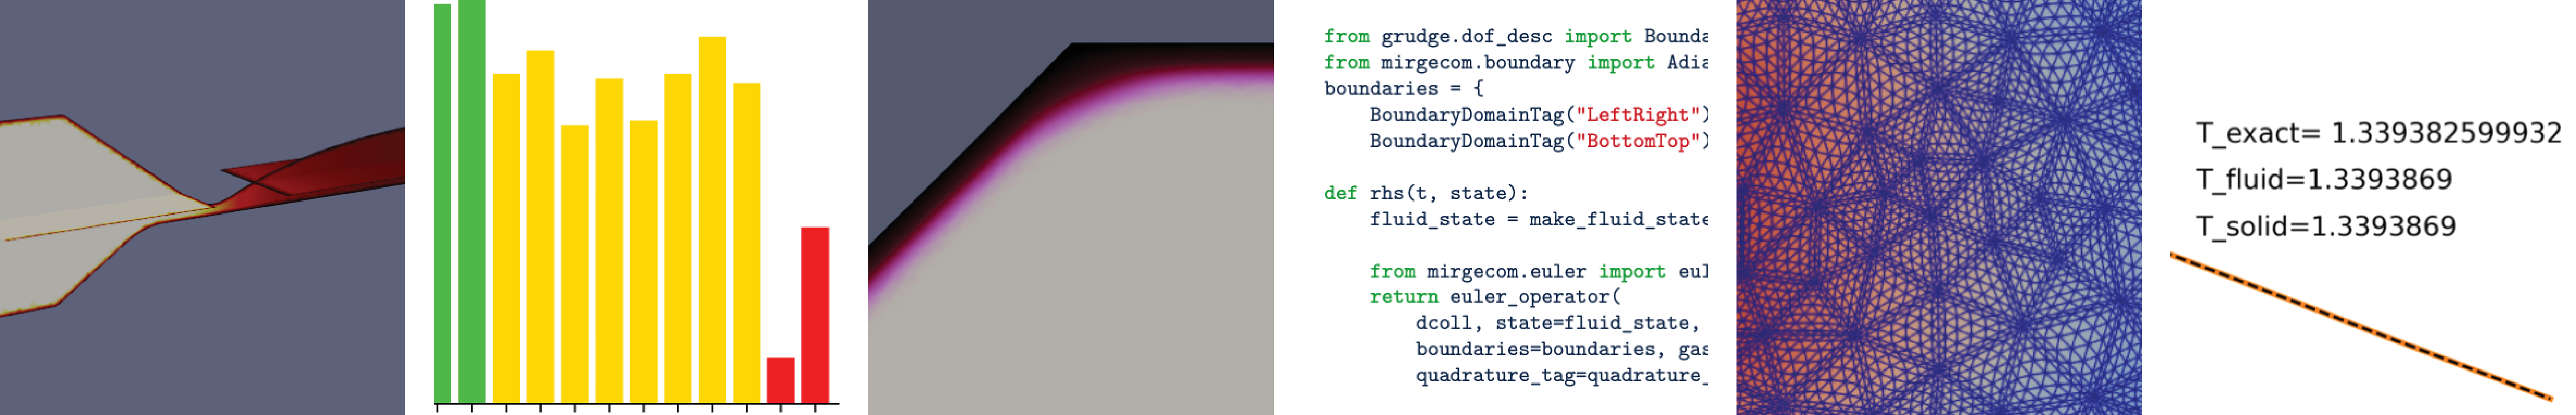
\includegraphics[width=0.7\textwidth]{Figures/coverart-sim.pdf}
\end{center}
\hrule

\vspace*{0.1in}
\hfill\cPI{Mike Campbell} \rPI{(CS)}  % \\
%\ \hbox{}\hfill\cPI{Matt Smith} \rPI{(NCSA)}\\
%\ \hbox{}\hfill\cPI{Mike Campbell} \rPI{(NCSA)}\\
%\ \hbox{}\hfill\cPI{Mike Anderson} \rPI{(NCSA)}

\end{frame}
%======================================================================

%======================================================================
%\begin{frame}[fragile]\frametitle{Outline}
%  \begin{tabular}{m{8cm}m{6cm}}
%  \begin{itemize}
%    \setlength{\itemsep}{0.0in}
%    \item Y2/Y3 Simulation infrastructure\prj{\tiny}{M.~Smith}
%      \begin{itemize}
%        \item How-to guide to \mirgecom
%        \item Wall modeling and coupling
%        \item Distributed DAG discussion
%      \end{itemize}
%  \end{itemize}
%  &
%  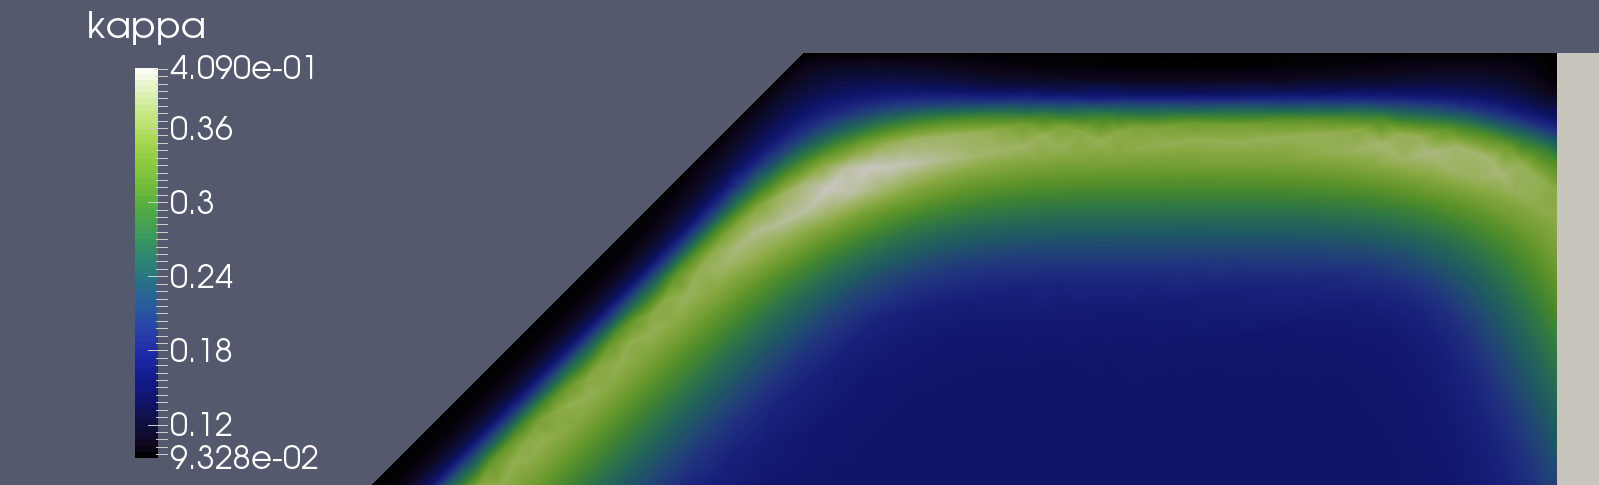
\includegraphics[width=6cm]{./Figures/smith/wall_kappa-clip.png}
%  \\[0cm]
%  \begin{itemize}
%    \setlength{\itemsep}{0.0in}
%    \item \mirgecom{} Performance \prj{\tiny}{M.~Campbell}
%      \begin{itemize}
%        \item Verification overview: testing, coverage
%        \item Performance highlights: scaling, monitoring
%      \end{itemize}
%  \end{itemize}
%  &
%  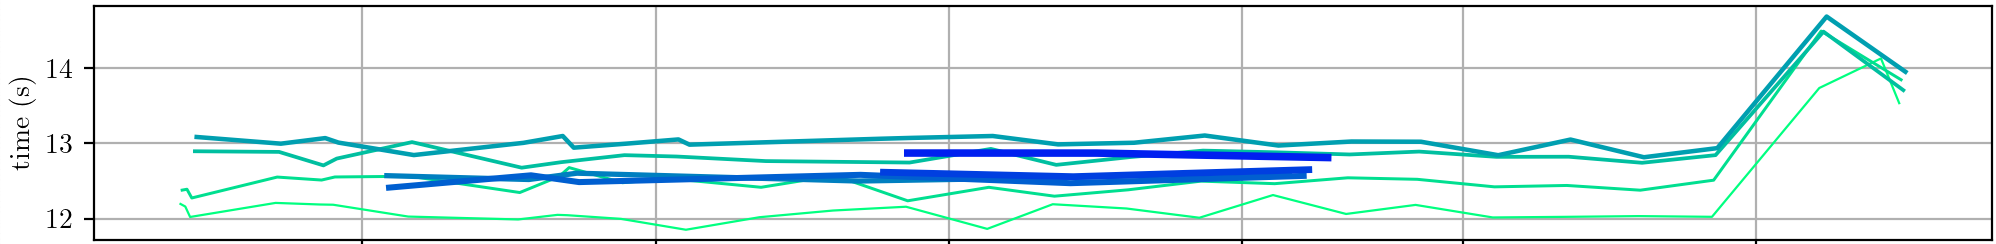
\includegraphics[width=6cm]{./Figures/timing-clip.png}
%  \\
%  \begin{itemize}
%    \setlength{\itemsep}{0.2in}
%    \item Prediction results\prj{\tiny}{M.~Anderson}
%      \begin{itemize}
%        \item Simulation status for Y3
%        \item Parsl, workflow plans \prj{\tiny}{Doug Friedel}
%      \end{itemize}
%  \end{itemize}
%  &
%  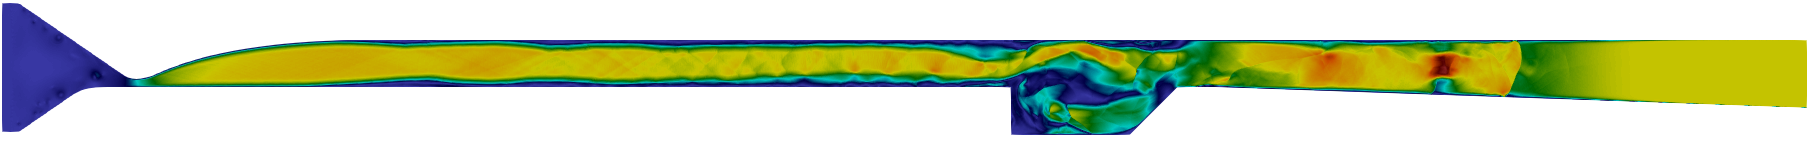
\includegraphics[width=6cm]{./Figures/Noslip_isolator_clipped.png}
%  \\
%  \begin{itemize}
%    \setlength{\itemsep}{0.2in}
%    \item Summary and risks \prj{\tiny}{Freund, Olson}
%  \end{itemize}
%  &
%  \end{tabular}
%\end{frame}
%======================================================================


% LukeO rip-off
\tikzstyle{c_mirgecom}   = []
\tikzstyle{c_meshmode}   = []
\tikzstyle{c_grudge}     = []
\tikzstyle{c_loopy}      = []
\tikzstyle{c_pytato}     = []
\tikzstyle{c_pyopencl}   = []
\tikzstyle{c_modepy}     = []
\tikzstyle{c_pymbolic}   = []
\tikzstyle{c_pocl}       = []
\tikzstyle{c_arraycontext} = []
\newcommand{\softwaredeps}{
  \tikzstyle{every path} = [line width=0.3pt,black!70]
  \tikzstyle{every node} = [scale=1.5,IllinoisBlue, line width=1pt]
  \begin{tikzpicture}[>=latex',line join=bevel,scale=0.34,
                      transform shape]
      %%
\node (mirgecom) at (306.3bp,522.0bp) [draw,ellipse,c_mirgecom] {mirgecom};
  \node (meshmode) at (198.3bp,378.0bp) [draw,ellipse,c_meshmode] {meshmode};
  \node (grudge) at (275.3bp,450.0bp) [draw,ellipse,c_grudge] {grudge};
  \node (loopy) at (300.3bp,162.0bp) [draw,ellipse,c_loopy] {loopy};
  \node (pytato) at (398.3bp,234.0bp) [draw,ellipse,c_pytato] {pytato};
  \node (pyopencl) at (82.3bp,90.0bp) [draw,ellipse,c_pyopencl] {pyopencl};
  \node (modepy) at (194.3bp,306.0bp) [draw,ellipse,c_modepy] {modepy};
  \node (arraycontext) at (82.3bp,306.0bp) [draw,ellipse,c_arraycontext] {arraycontext};
  \node (pymbolic) at (339.3bp,90.0bp) [draw,ellipse,c_pymbolic] {pymbolic};
  \node (pocl) at (82.3bp,18.0bp) [draw,ellipse,c_pocl] {pocl};
  \draw [->] (mirgecom) ..controls (263.07bp,497.84bp) and (243.93bp,484.43bp)  .. (231.3bp,468.0bp) .. controls (217.23bp,449.7bp) and (208.68bp,424.78bp)  .. (meshmode);
  \draw [->] (mirgecom) ..controls (295.22bp,495.97bp) and (290.85bp,486.12bp)  .. (grudge);
  \draw [->] (mirgecom) ..controls (322.13bp,477.36bp) and (338.3bp,424.99bp)  .. (338.3bp,379.0bp) .. controls (338.3bp,379.0bp) and (338.3bp,379.0bp)  .. (338.3bp,305.0bp) .. controls (338.3bp,263.41bp) and (322.9bp,217.22bp)  .. (loopy);
  \draw [->] (mirgecom) ..controls (333.95bp,495.26bp) and (345.45bp,482.01bp)  .. (352.3bp,468.0bp) .. controls (386.02bp,399.05bp) and (395.02bp,307.18bp)  .. (pytato);
  \draw [->] (meshmode) ..controls (224.34bp,350.64bp) and (235.59bp,337.39bp)  .. (243.3bp,324.0bp) .. controls (256.77bp,300.58bp) and (279.94bp,228.93bp)  .. (loopy);
  \draw [->] (meshmode) ..controls (105.37bp,361.51bp) and (34.495bp,345.65bp)  .. (18.3bp,324.0bp) .. controls (-29.855bp,259.62bp) and (29.958bp,161.05bp)  .. (pyopencl);
  \draw [->] (meshmode) ..controls (196.87bp,351.98bp) and (196.34bp,342.71bp)  .. (modepy);
  \draw [->] (meshmode) ..controls (156.9bp,352.02bp) and (134.42bp,338.45bp)  .. (arraycontext);
  \draw [->] (grudge) ..controls (248.31bp,424.47bp) and (234.95bp,412.31bp)  .. (meshmode);
  \draw [->] (grudge) ..controls (280.96bp,384.29bp) and (292.77bp,249.18bp)  .. (loopy);
  \draw [->] (loopy) ..controls (237.05bp,140.69bp) and (169.33bp,118.95bp)  .. (pyopencl);
  \draw [->] (loopy) ..controls (314.0bp,136.4bp) and (319.79bp,126.02bp)  .. (pymbolic);
  \draw [->] (pyopencl) ..controls (82.3bp,63.983bp) and (82.3bp,54.712bp)  .. (pocl);
  \draw [->] (arraycontext) ..controls (146.51bp,263.17bp) and (228.67bp,209.66bp)  .. (loopy);
  \draw [->] (arraycontext) ..controls (82.3bp,250.83bp) and (82.3bp,163.18bp)  .. (pyopencl);
  \draw [->] (arraycontext) ..controls (130.09bp,291.77bp) and (137.92bp,289.77bp)  .. (145.3bp,288.0bp) .. controls (219.86bp,270.15bp) and (307.59bp,252.52bp)  .. (pytato);
  \draw [->] (pytato) ..controls (364.12bp,208.58bp) and (343.5bp,193.86bp)  .. (loopy);
  \draw [->] (pytato) ..controls (381.14bp,191.71bp) and (362.22bp,146.17bp)  .. (pymbolic);
%

  \end{tikzpicture}
}
%\newcommand{\softwaredeps}{
%  \tikzstyle{every path} = [thick,black]

\begin{tikzpicture}[>=latex',line join=bevel,scale=0.5,transform shape]
  \node[c_mirgecom] (mirgecom) at (128.0bp,394.0bp) [draw,ellipse] {mirgecom};
  \node[c_meshmode] (meshmode) at (66.0bp,250.0bp) [draw,ellipse] {meshmode};
  \node[c_grudge] (grudge) at (101.0bp,322.0bp) [draw,ellipse] {grudge};
  \node[c_loopy] (loopy) at (165.0bp,178.0bp) [draw,ellipse] {loopy};
  \node[c_pytato] (pytato) at (206.0bp,250.0bp) [draw,ellipse] {pytato};
  \node[c_pyopencl] (pyopencl) at (89.0bp,106.0bp) [draw,ellipse] {pyopencl};
  \node[c_modepy] (modepy) at (56.0bp,178.0bp) [draw,ellipse] {modepy};
  \node[c_pymbolic] (pymbolic) at (194.0bp,106.0bp) [draw,ellipse] {pymbolic};
  \node[c_pocl] (pocl) at (89.0bp,34.0bp) [draw,ellipse] {pocl};
  \draw [->] (mirgecom) ..controls (83.575bp,370.85bp) and (65.825bp,357.6bp)  .. (57.0bp,340.0bp) .. controls (47.309bp,320.67bp) and (50.82bp,296.05bp)  .. (meshmode);
  \draw [->] (mirgecom) ..controls (118.38bp,368.06bp) and (114.63bp,358.33bp)  .. (grudge);
  \draw [->] (mirgecom) ..controls (137.95bp,365.74bp) and (142.3bp,352.27bp)  .. (145.0bp,340.0bp) .. controls (155.24bp,293.54bp) and (160.68bp,238.3bp)  .. (loopy);
  \draw [->] (mirgecom) ..controls (145.03bp,365.67bp) and (153.18bp,352.19bp)  .. (160.0bp,340.0bp) .. controls (171.75bp,319.0bp) and (184.24bp,294.7bp)  .. (pytato);
  \draw [->] (meshmode) ..controls (102.68bp,223.07bp) and (122.14bp,209.3bp)  .. (loopy);
  \draw [->] (meshmode) ..controls (90.689bp,223.14bp) and (100.44bp,209.89bp)  .. (105.0bp,196.0bp) .. controls (111.74bp,175.46bp) and (106.6bp,151.26bp)  .. (pyopencl);
  \draw [->] (meshmode) ..controls (62.426bp,223.98bp) and (61.102bp,214.71bp)  .. (modepy);
  \draw [->] (grudge) ..controls (88.625bp,296.25bp) and (83.61bp,286.22bp)  .. (meshmode);
  \draw [->] (grudge) ..controls (113.31bp,293.86bp) and (119.52bp,280.15bp)  .. (125.0bp,268.0bp) .. controls (134.58bp,246.76bp) and (145.41bp,222.66bp)  .. (loopy);
  \draw [->] (loopy) ..controls (138.91bp,152.97bp) and (125.17bp,140.32bp)  .. (pyopencl);
  \draw [->] (loopy) ..controls (175.22bp,152.34bp) and (179.32bp,142.43bp)  .. (pymbolic);
  \draw [->] (pyopencl) ..controls (89.0bp,79.983bp) and (89.0bp,70.712bp)  .. (pocl);
  \draw [->] (pytato) ..controls (191.47bp,224.19bp) and (185.2bp,213.49bp)  .. (loopy);
  \draw [->] (pytato) ..controls (207.38bp,213.92bp) and (207.7bp,184.89bp)  .. (205.0bp,160.0bp) .. controls (204.07bp,151.46bp) and (202.41bp,142.26bp)  .. (pymbolic);
  %\draw[red!50] (0,0) rectangle (230pt, 387.0pt);
\end{tikzpicture}

%}
\begin{frame}\frametitle{Outline}
\begin{minipage}[T]{0.45\textwidth}
  \begin{itemize}
    \item \textbf{MIRGE-Com Overview}
    \item \textbf{Performance \& Scalability}
    \item \textbf{Code Challenges}
    %    \begin{itemize}
    %        \item Partitioning \& DAG Splat Issues
    %        \item Mesh Processing Complexities
    %        \item DAG Complexity with physics development/capabilities
    %        \item Upcoming Threats \& Concerns
    %    \end{itemize}
    %  \end{itemize}
    \item \textbf{Conclusion \& Future Directions}
    %\begin{itemize}
    %    \item Upcoming Review Priorities
    %    \item Vision \& Long-Term Goals
    %\end{itemize}
  \end{itemize}
\end{minipage}
\hfill
\begin{minipage}[T]{0.45\textwidth}
  \centering
  \tikzstyle{c_mirgecom}=[draw=myOrange, line width=0.5mm]
  \softwaredeps%
\end{minipage}
  \url{https://github.com/illinois-ceesd/mirgecom/}
\end{frame}

\begin{frame}
    \centering
    \Large
    \textbf{MIRGE-Com in Y3}
    % \begin{itemize}
    %    \item Architecture Overview
    %    \item Supported Features, Physics
    %    \item Development Overview (production eliminiation)
    % \end{itemize}
\end{frame}

\begin{frame}\frametitle{Architecture Overview}
  \begin{center}
  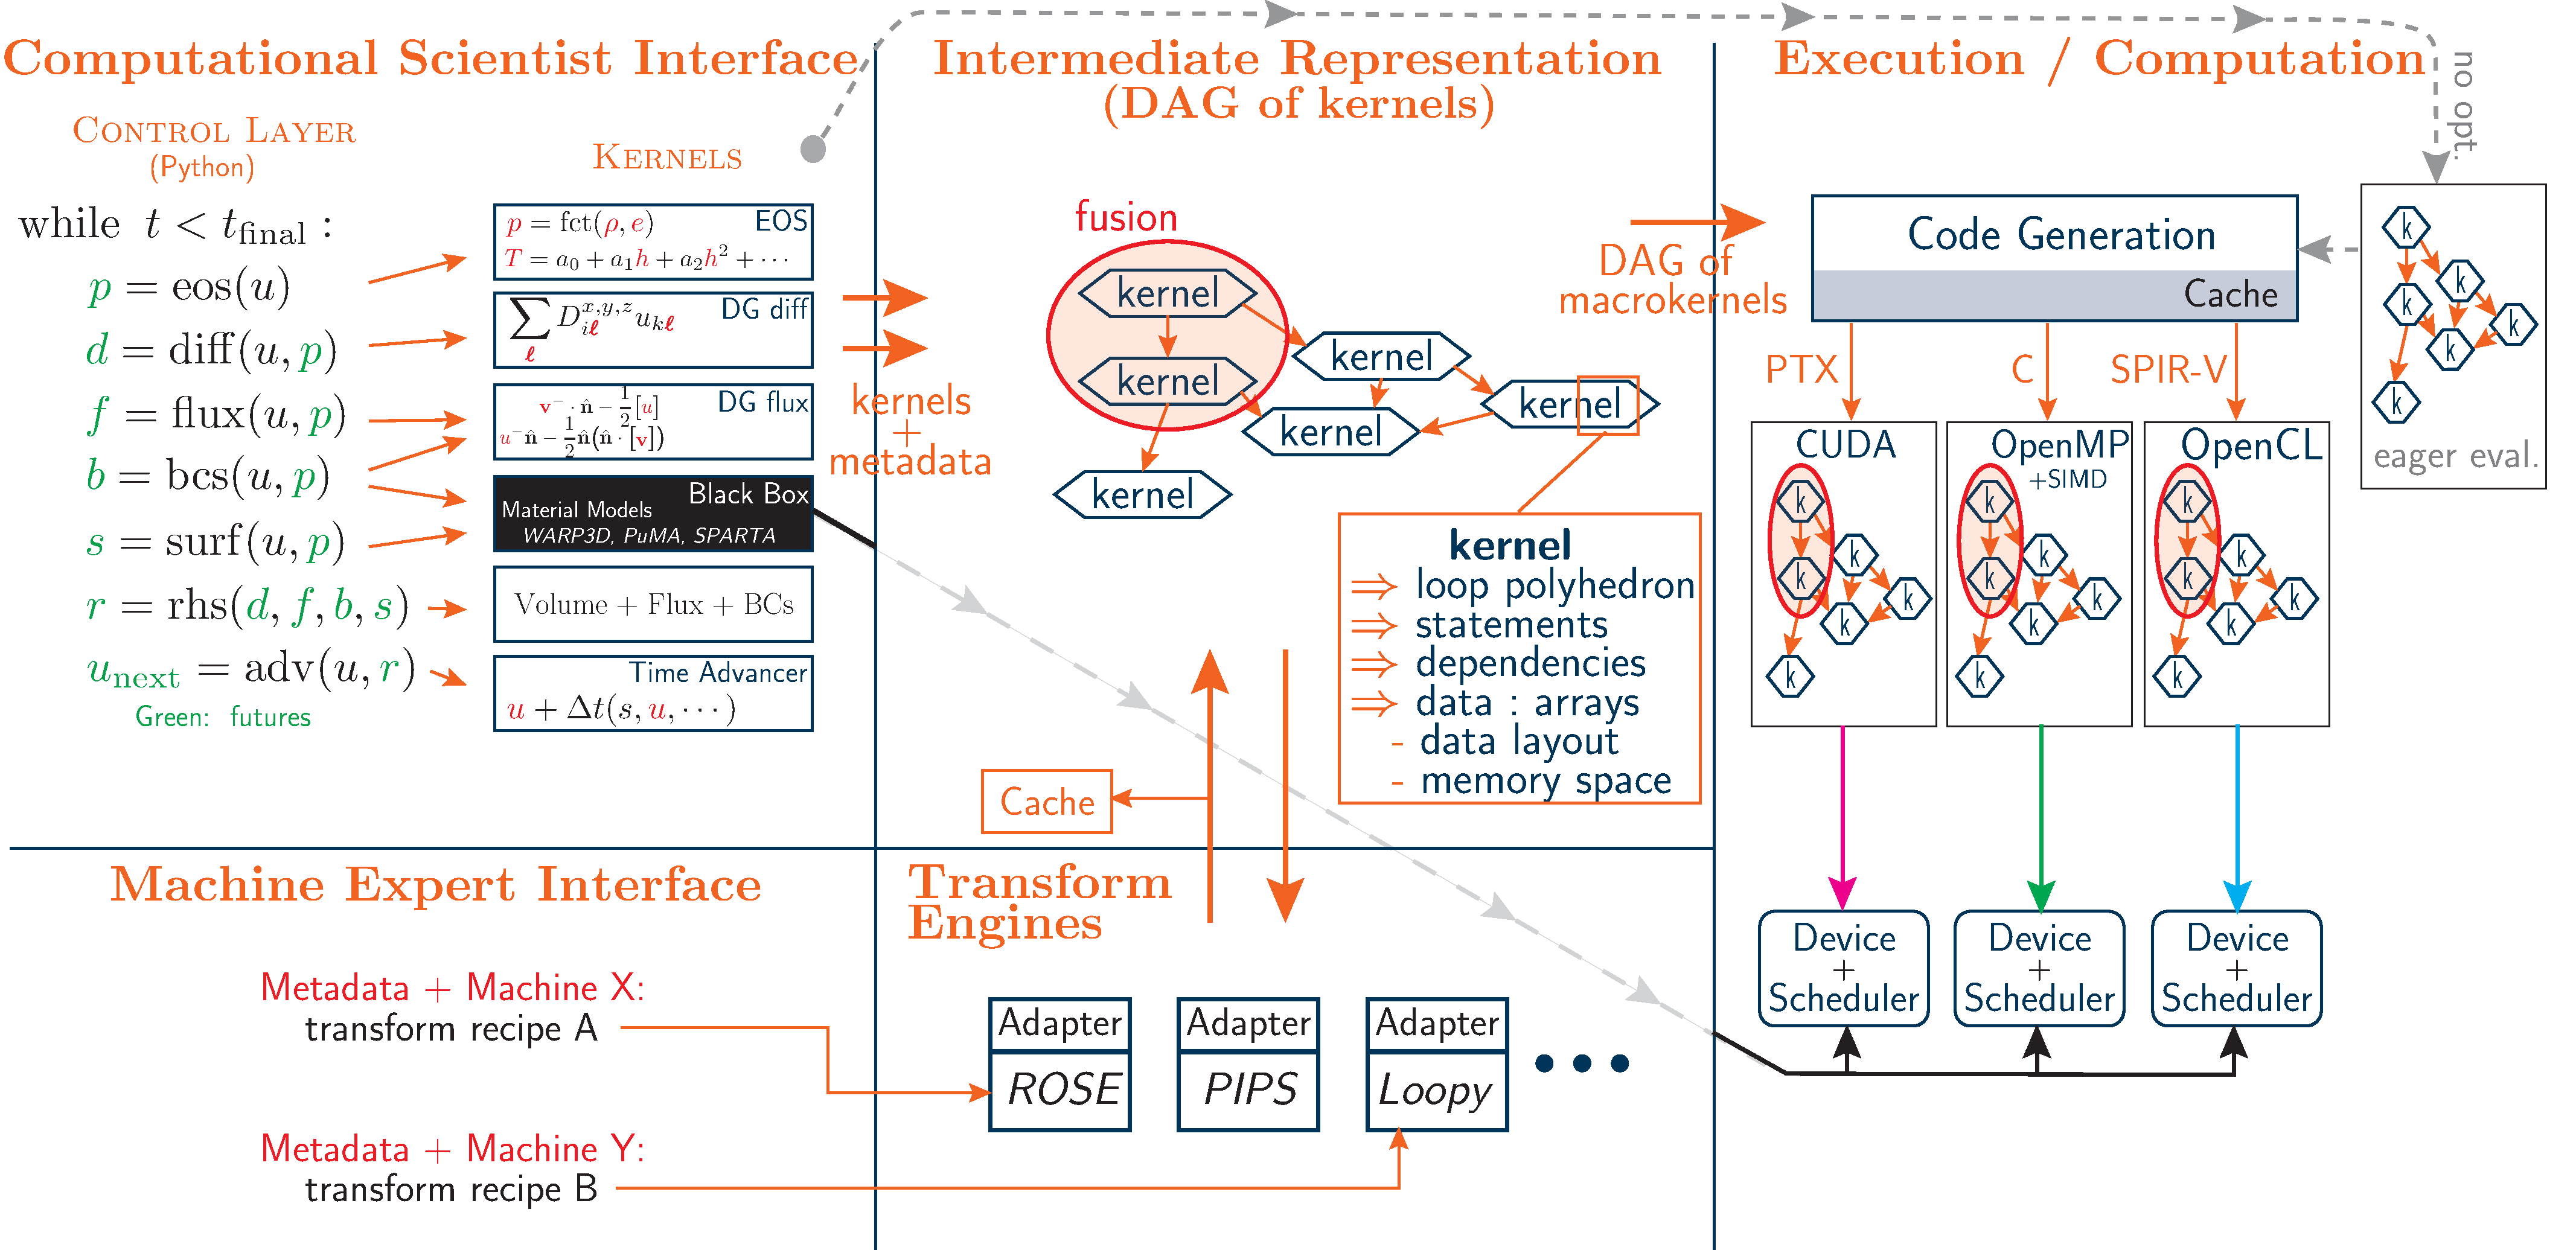
\includegraphics[width=.95\textwidth]{Figures/controllayer-new.pdf}
  % \vspace*{-5pt}
  \end{center}
\end{frame}

\begin{frame}\frametitle{Simulation Infrastructure}
\begin{multicols}{2}
\begin{itemize}
\item Infrastructure provides:
  \begin{itemize}
  \item DG operators (e.g., mass, stiffness, grad, div)% , ($\mathcal{S}$)
  \item Multiple parallel discrete geometries \prj{\tiny}{M.~Smith}
   % and other machinery, spectral domain access, etc, interior\_trace\_pair - selects all interior faces
  \item Compute device access
  \item Symbolic infrastructure - great for verification
  \end{itemize}
\end{itemize}
\columnbreak
\begin{itemize}
\item \textit{MIRGE-Com} library provides:
  \begin{itemize}
  \item Conservation-law-specific data structures
  \item Simulation / driver API
  \item Prediction-relevant
    \begin{itemize}
    \item RHS operators
    \item Model-specific constructs (e.g., EOS, transport, reactions)
    \item Boundary and numerical fluxes
    \end{itemize}
  \end{itemize}
\end{itemize}
\end{multicols}
\vspace{-10pt}
\lstinputlisting[style=kkcodestyle, basicstyle=\tiny, language=Python]{Figures/mtc/rhs_sample.py}
%\begin{multicols}{2}
%  \lstinputlisting[style=kkcodestyle, basicstyle=\tiny, language=Python]{Figures/mtc/rhs_sample2.py}
%\columnbreak
%  \lstinputlisting[style=kkcodestyle, basicstyle=\tiny, language=Python]{Figures/mtc/rhs_sample3.py}
%\end{multicols}
\end{frame}



\begin{frame}\frametitle{Prediction-supporting Development}
  \begin{center}
  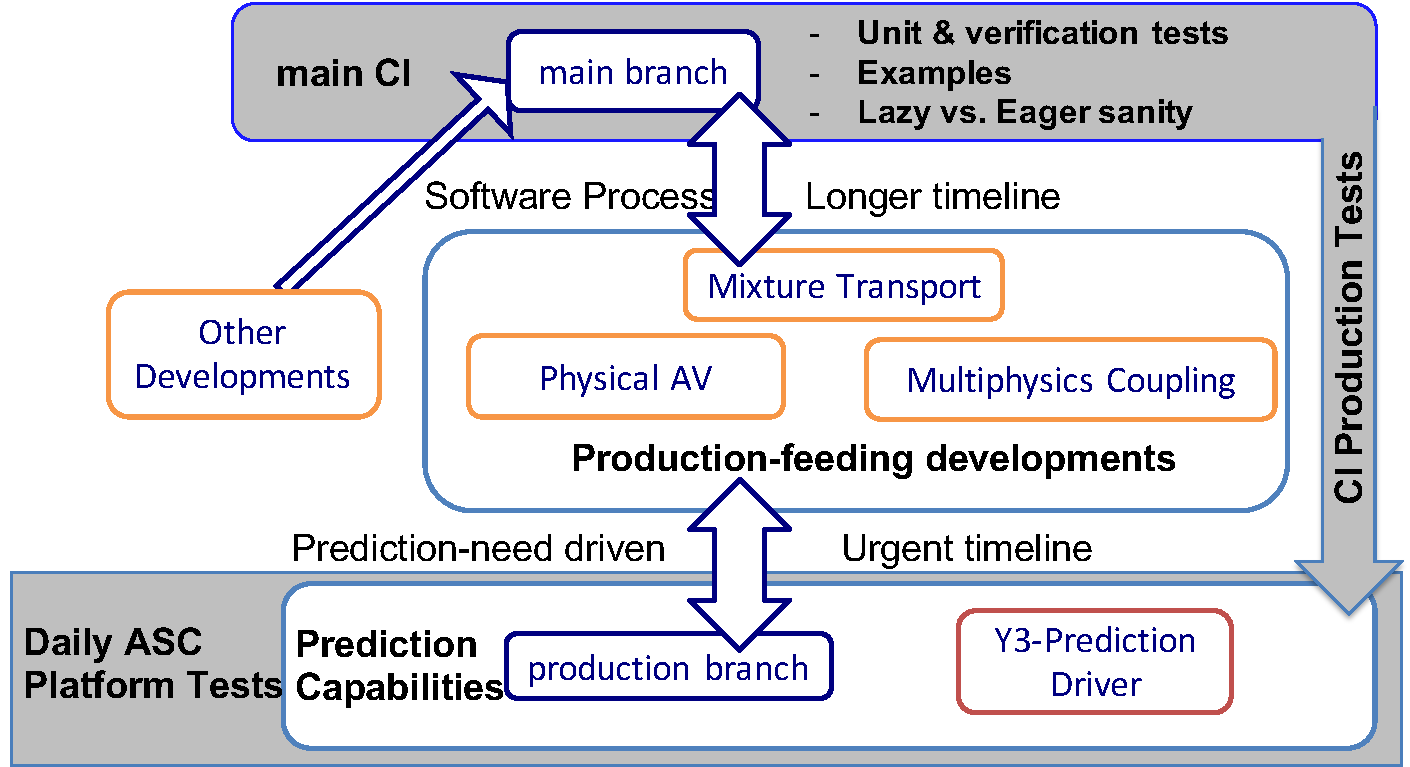
\includegraphics[width=.65\textwidth]{Figures/mtc/PredictionSupportinDevel3.pdf}
  \vspace*{-5pt}
  \end{center}
  \begin{center}
  % \vspace*{-15pt}
  \begin{itemize}
  \item Prediction-supporting development process
  \item Prediction-targeted testing mechanism
  \item Continuous integration and daily ASC platform testing
  \end{itemize}
  \end{center}
  \begin{tikzpicture}[remember picture, overlay]
    \fill <2> [fill=white, opacity=0.8] (current page.south west) + (0.5,0.5) rectangle (12.5,7.5);
    \node <2> [inner sep=0pt] at (current page.center) {
      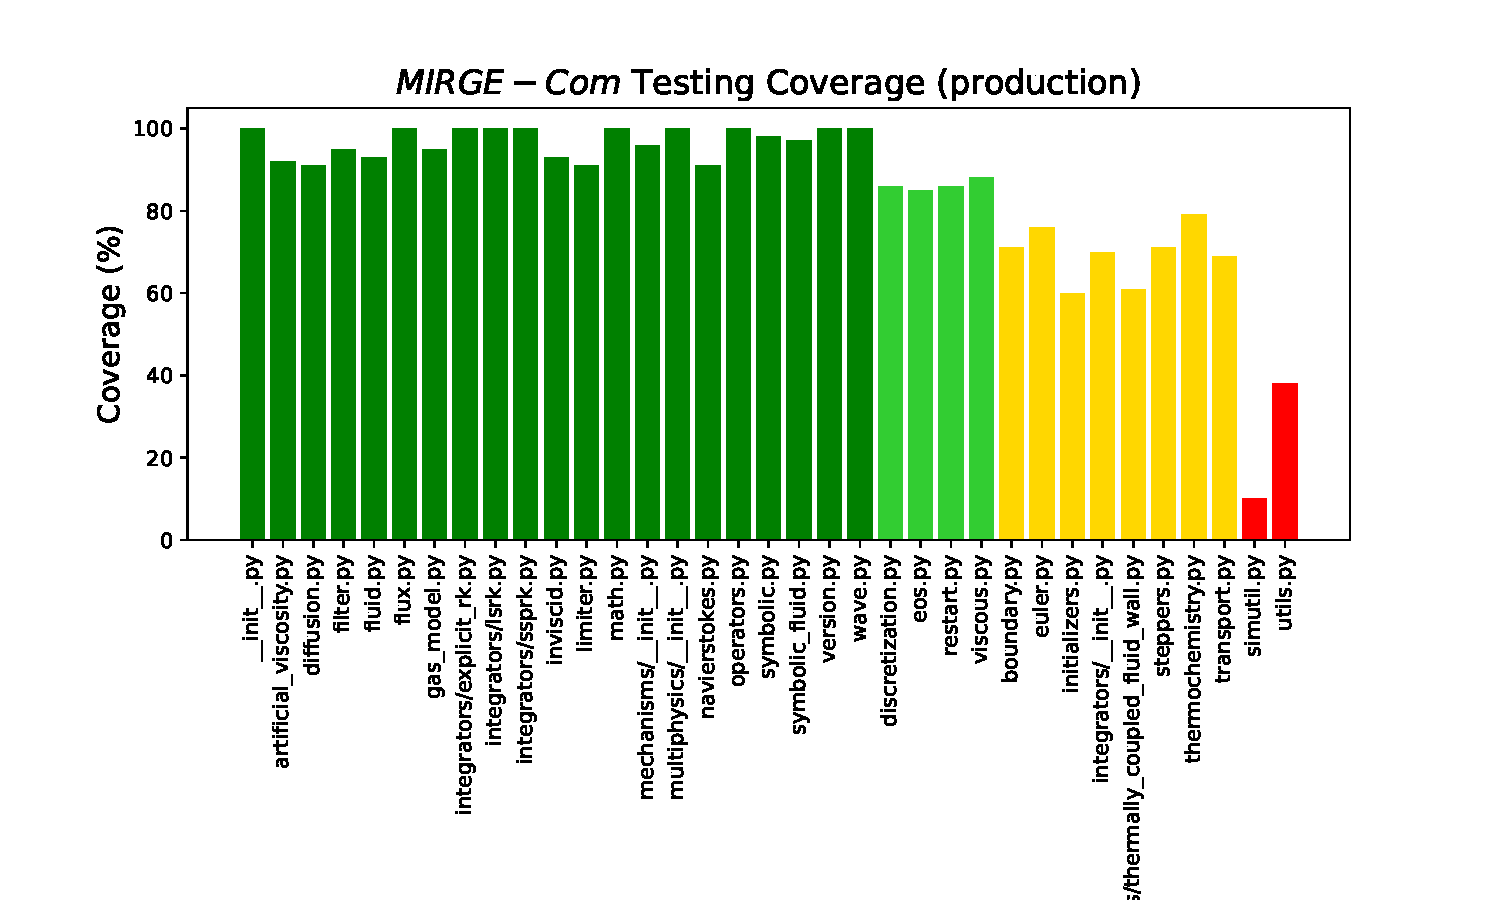
\includegraphics[width=.9\textwidth]{Figures/mtc/coverage_plot_production.pdf}
    };
  \end{tikzpicture}
\end{frame}


\begin{frame}\frametitle{Prediction-supporting Development}
  \begin{center}
  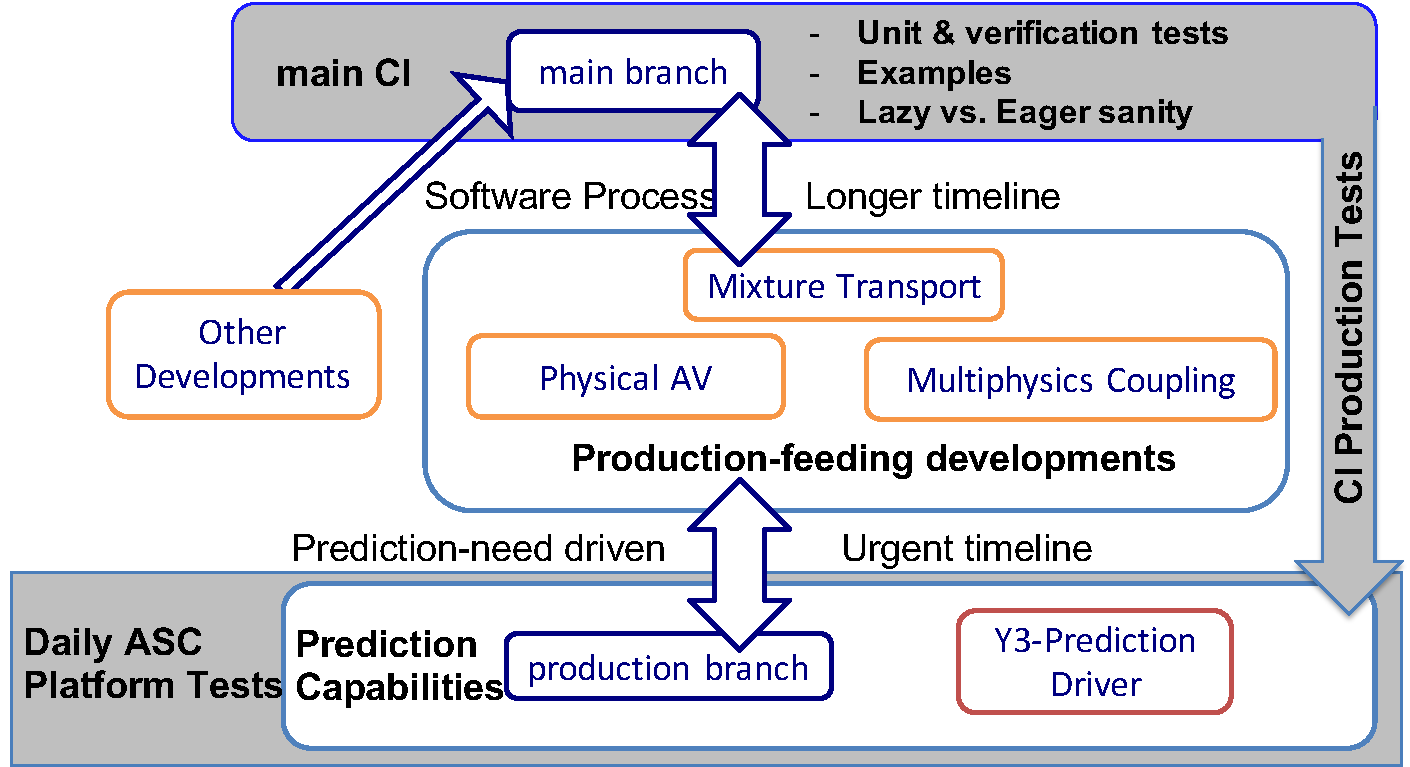
\includegraphics[width=.65\textwidth]{Figures/mtc/PredictionSupportinDevel3.pdf}
  \vspace*{-5pt}
  \end{center}
  \begin{center}
  % \vspace*{-15pt}
  \begin{itemize}
  \item Prediction-supporting development process
  \item Prediction-targeted testing mechanism
  \item Continuous integration and daily ASC platform testing
  \end{itemize}
  \end{center}
  \begin{tikzpicture}[remember picture, overlay]
    \fill <2> [fill=white, opacity=0.8] (current page.south west) + (0.5,0.5) rectangle (12.5,7.5);
    \node <2> [inner sep=0pt] at (current page.center) {
      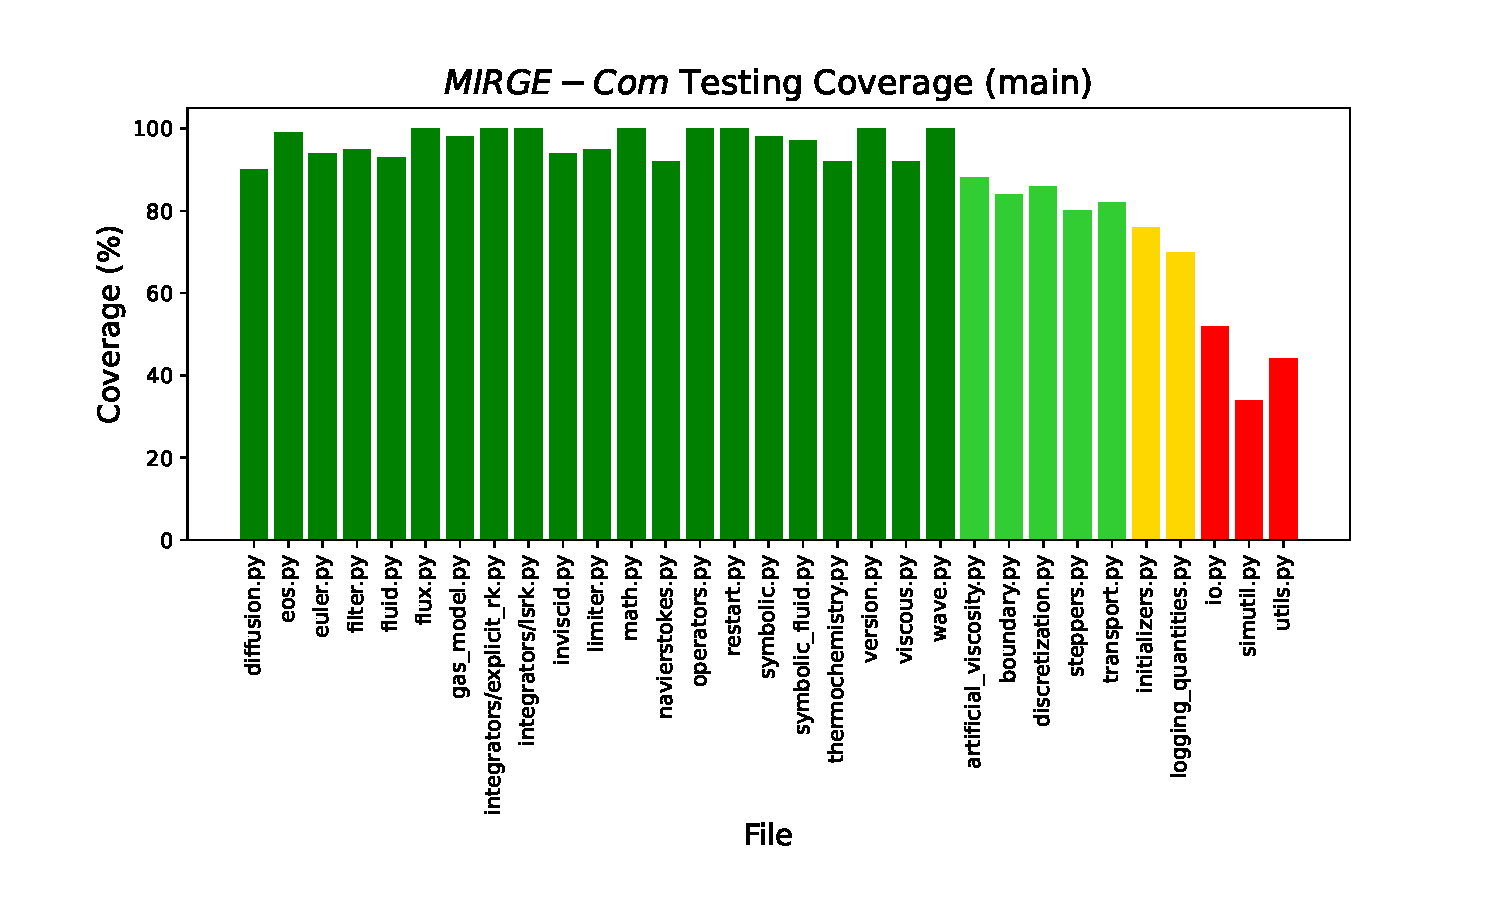
\includegraphics[width=.9\textwidth]{Figures/mtc/coverage_plot_main.pdf}
    };
  \end{tikzpicture}
\end{frame}

\begin{frame}\frametitle{Prediction-supporting Development}
  \begin{center}
  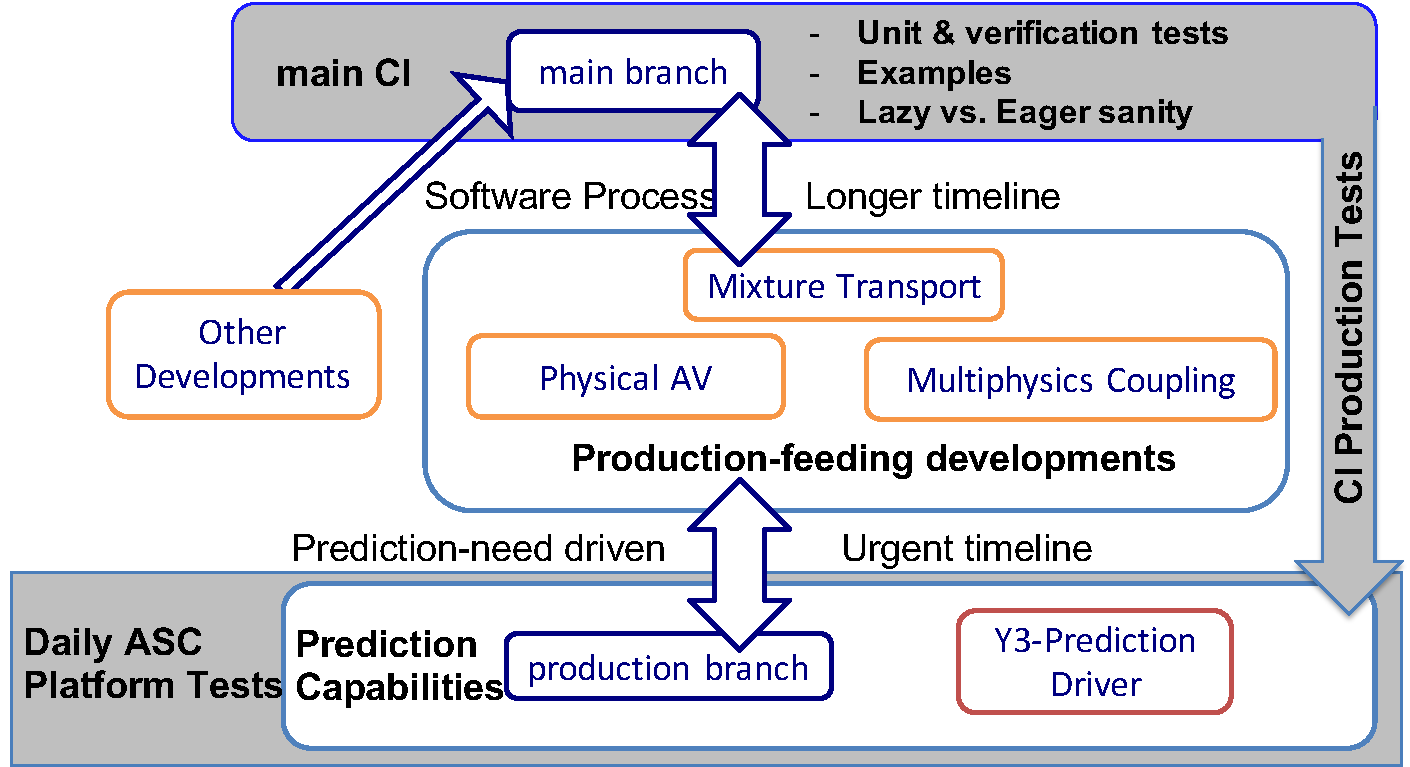
\includegraphics[width=.65\textwidth]{Figures/mtc/PredictionSupportinDevel3.pdf}
  \vspace*{-5pt}
  \end{center}
  \begin{center}
  % \vspace*{-15pt}
  \begin{itemize}
  \item Prediction-supporting development process
  \item Prediction-targeted testing mechanism
  \item Continuous integration and daily ASC platform testing
  \end{itemize}
  \end{center}
\end{frame}

%\begin{frame}\frametitle{Thermochemistry Verification in \mirgecom}
%\begin{center}
% Autoignition co-verification
%\end{center}
%\begin{itemize}
%   \item Ethylene/air mixture $(1500\mathtt{K}, \rho=\mathtt{const})$
%   \item \pyrometheus-predicted profiles match \textit{Cantera}
%   \item \pyrometheus{} with implicit time integration with \textit{CVODE}
%   \item \mirgecom{} with RK4, inviscid, quiescent
%\end{itemize}
%\begin{multicols}{2}
%    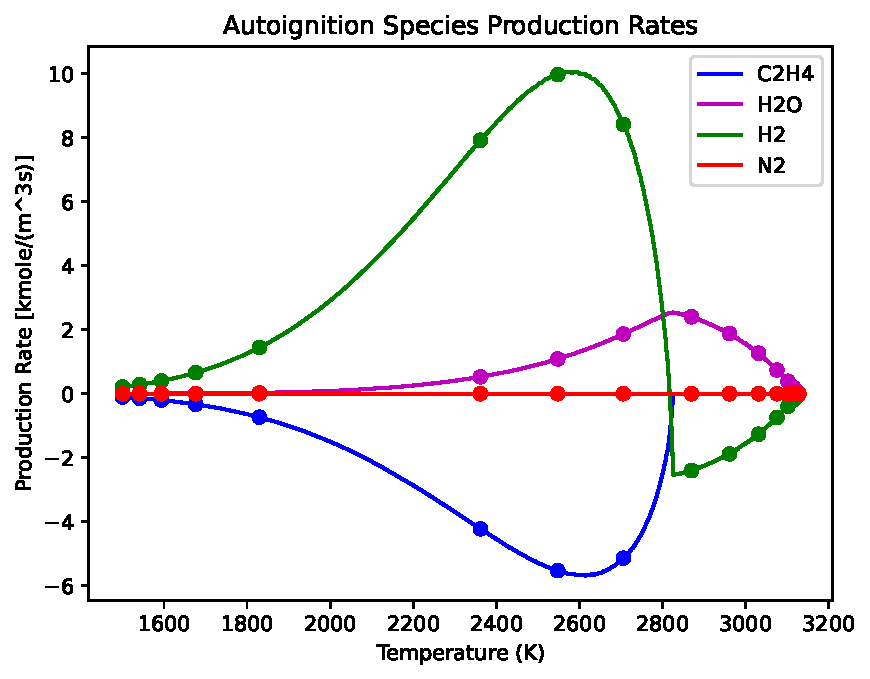
\includegraphics[width=.4\textwidth]{Figures/mtc/autoignition_rates.pdf}\\
%    \columnbreak
%    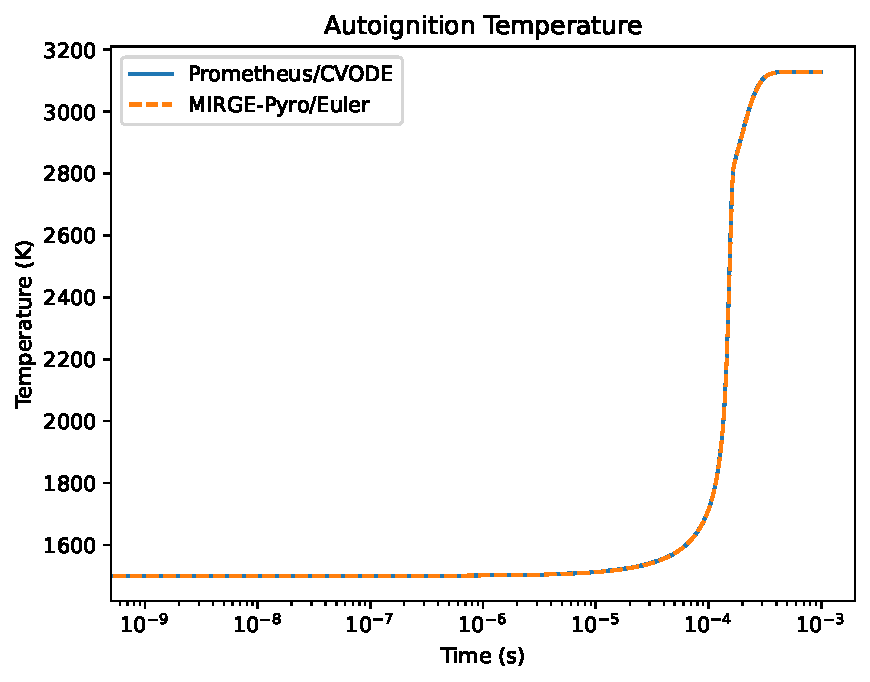
\includegraphics[width=.4\textwidth]{Figures/mtc/autoignition_temperature.pdf}
%  \end{multicols}
%\end{frame}

\begin{frame}
    \centering
    \Large
    \textbf{Performance \& Scalability}
    % Fundamentals
    % \begin{itemize}
    %    \item Strong Scaling: Fixed problem size, scaling resource
    %    \item Weak Scaling: Scaled problem size, fixed work/resource
    %    \item Versatility: Portability, resource options
    %\end{itemize}
    % MIRGE-Com scaling in Y3
    % \item \textbf{MIRGE-Com Scaling in Y3}
    % \begin{itemize}
    %    \item Why do we care?  (Enabling prediction!)
    %    \item Performance Snapshots
    %    \begin{itemize}
    %        \item Weak Scaling Achievements
    %        \item Strong Scaling Insights
    %        \item Lassen Monitoring Highlights
    %    \end{itemize}
\end{frame}

\begin{frame}\frametitle{Performance}
\begin{minipage}[t][0.4\textheight][t]{\textwidth}
\begin{center}
New: prediction-enabling performance
\end{center}
\begin{multicols}{2}
\begin{itemize}
\item Scaling as expected (mostly)
\item Small problems are expensive
\columnbreak
\item OOM: SVM/Unified memory \prj\tiny{07c, M.~Diener}
\item Mem growth: Garbage collection
\end{itemize}
%\item Absolute performance could be better
%\item Recent focus: memory growth
%\end{itemize}
\end{multicols}
\end{minipage}\vfill
\vspace{-20pt}
\begin{minipage}[t][0.4\textheight][t]{\textwidth}
\centering
%Grid Scaling\\
%\end{center}
%\begin{center}
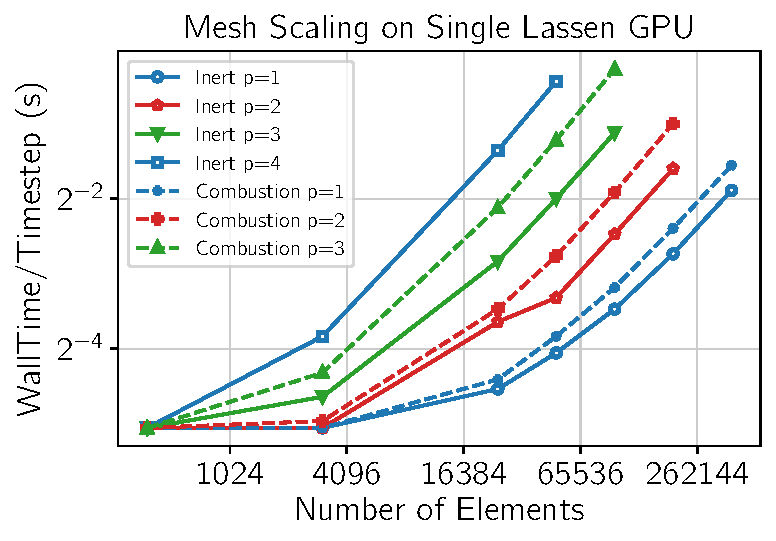
\includegraphics[width=.4\textwidth]{Figures/mtc/combozzle_gridscale.pdf}\hspace{30pt}
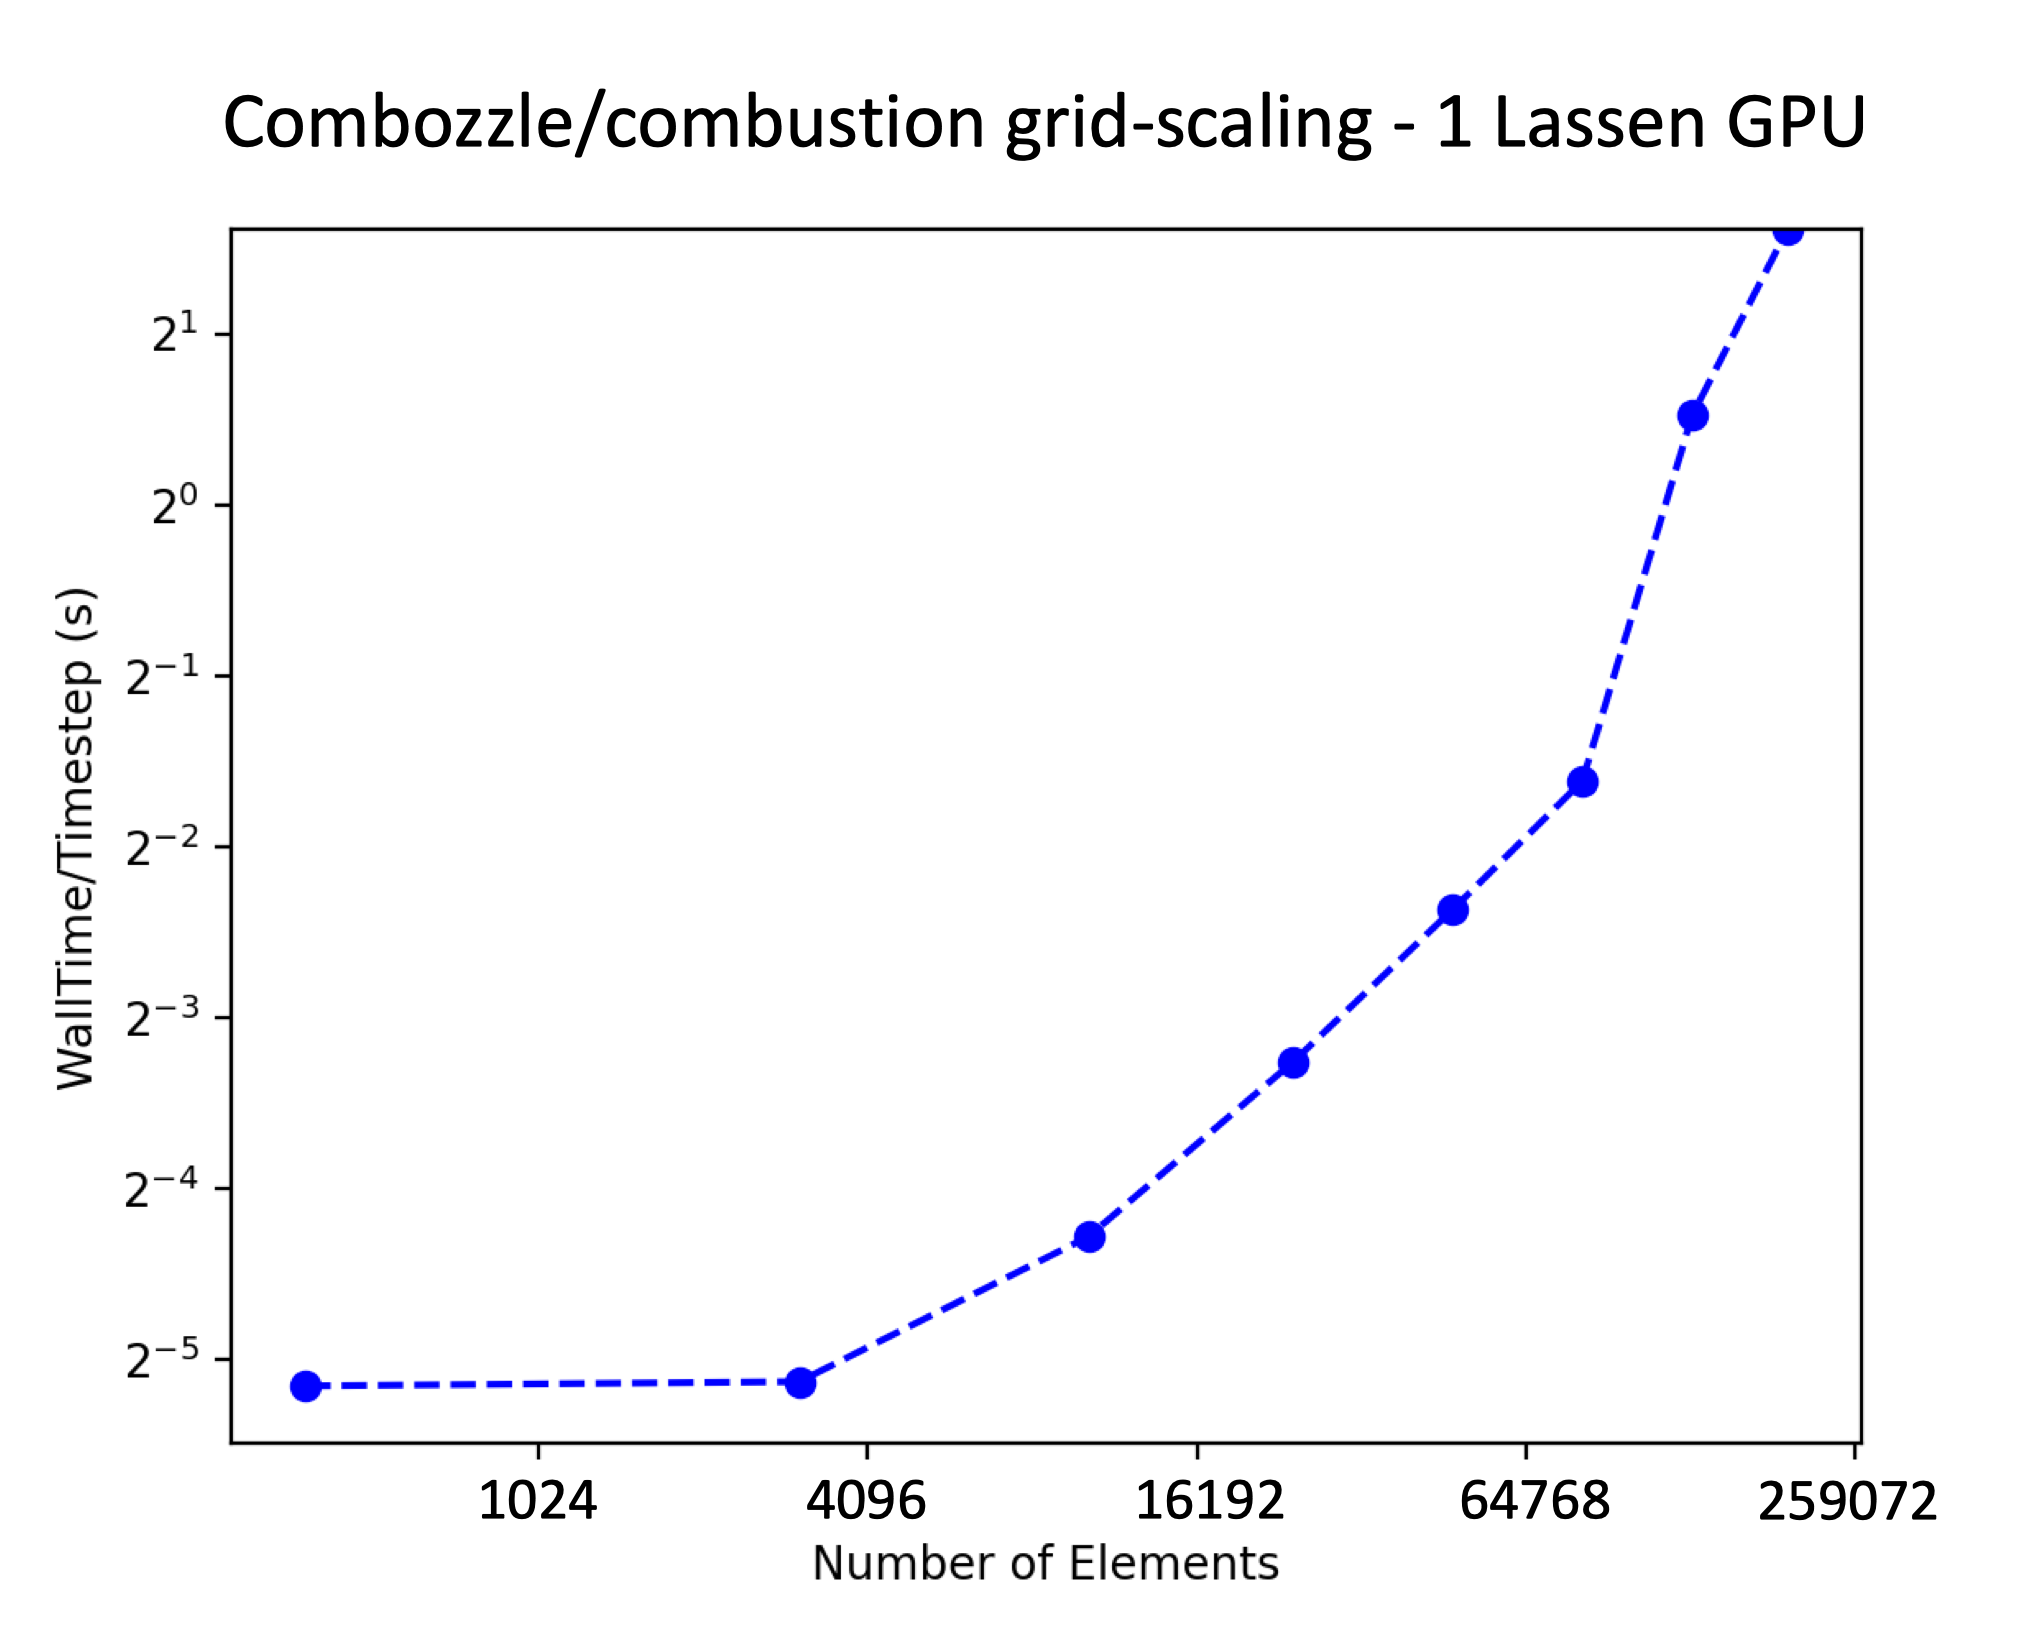
\includegraphics[width=.4\textwidth]{Figures/mtc/comboz_gridscale_svm.png}
\end{minipage}
\end{frame}


\begin{frame}\frametitle{Performance}
\begin{minipage}[t][0.4\textheight][t]{\textwidth}
\begin{center}
New: prediction-enabling performance
\end{center}
\begin{multicols}{2}
\begin{itemize}
\item DAG Splat: DAG for each boundary
\item Limits weak scaling - DAG for each neighbor
\columnbreak
\item Mitigation: Metis $\to$ 1D decomp
\item Real fix: Function calls in the DAG \prj\tiny{Kaushik Kulkarni}
\end{itemize}
\end{multicols}
\end{minipage}\vfill
\vspace{-20pt}
\begin{minipage}[t][0.4\textheight][t]{\textwidth}
\centering
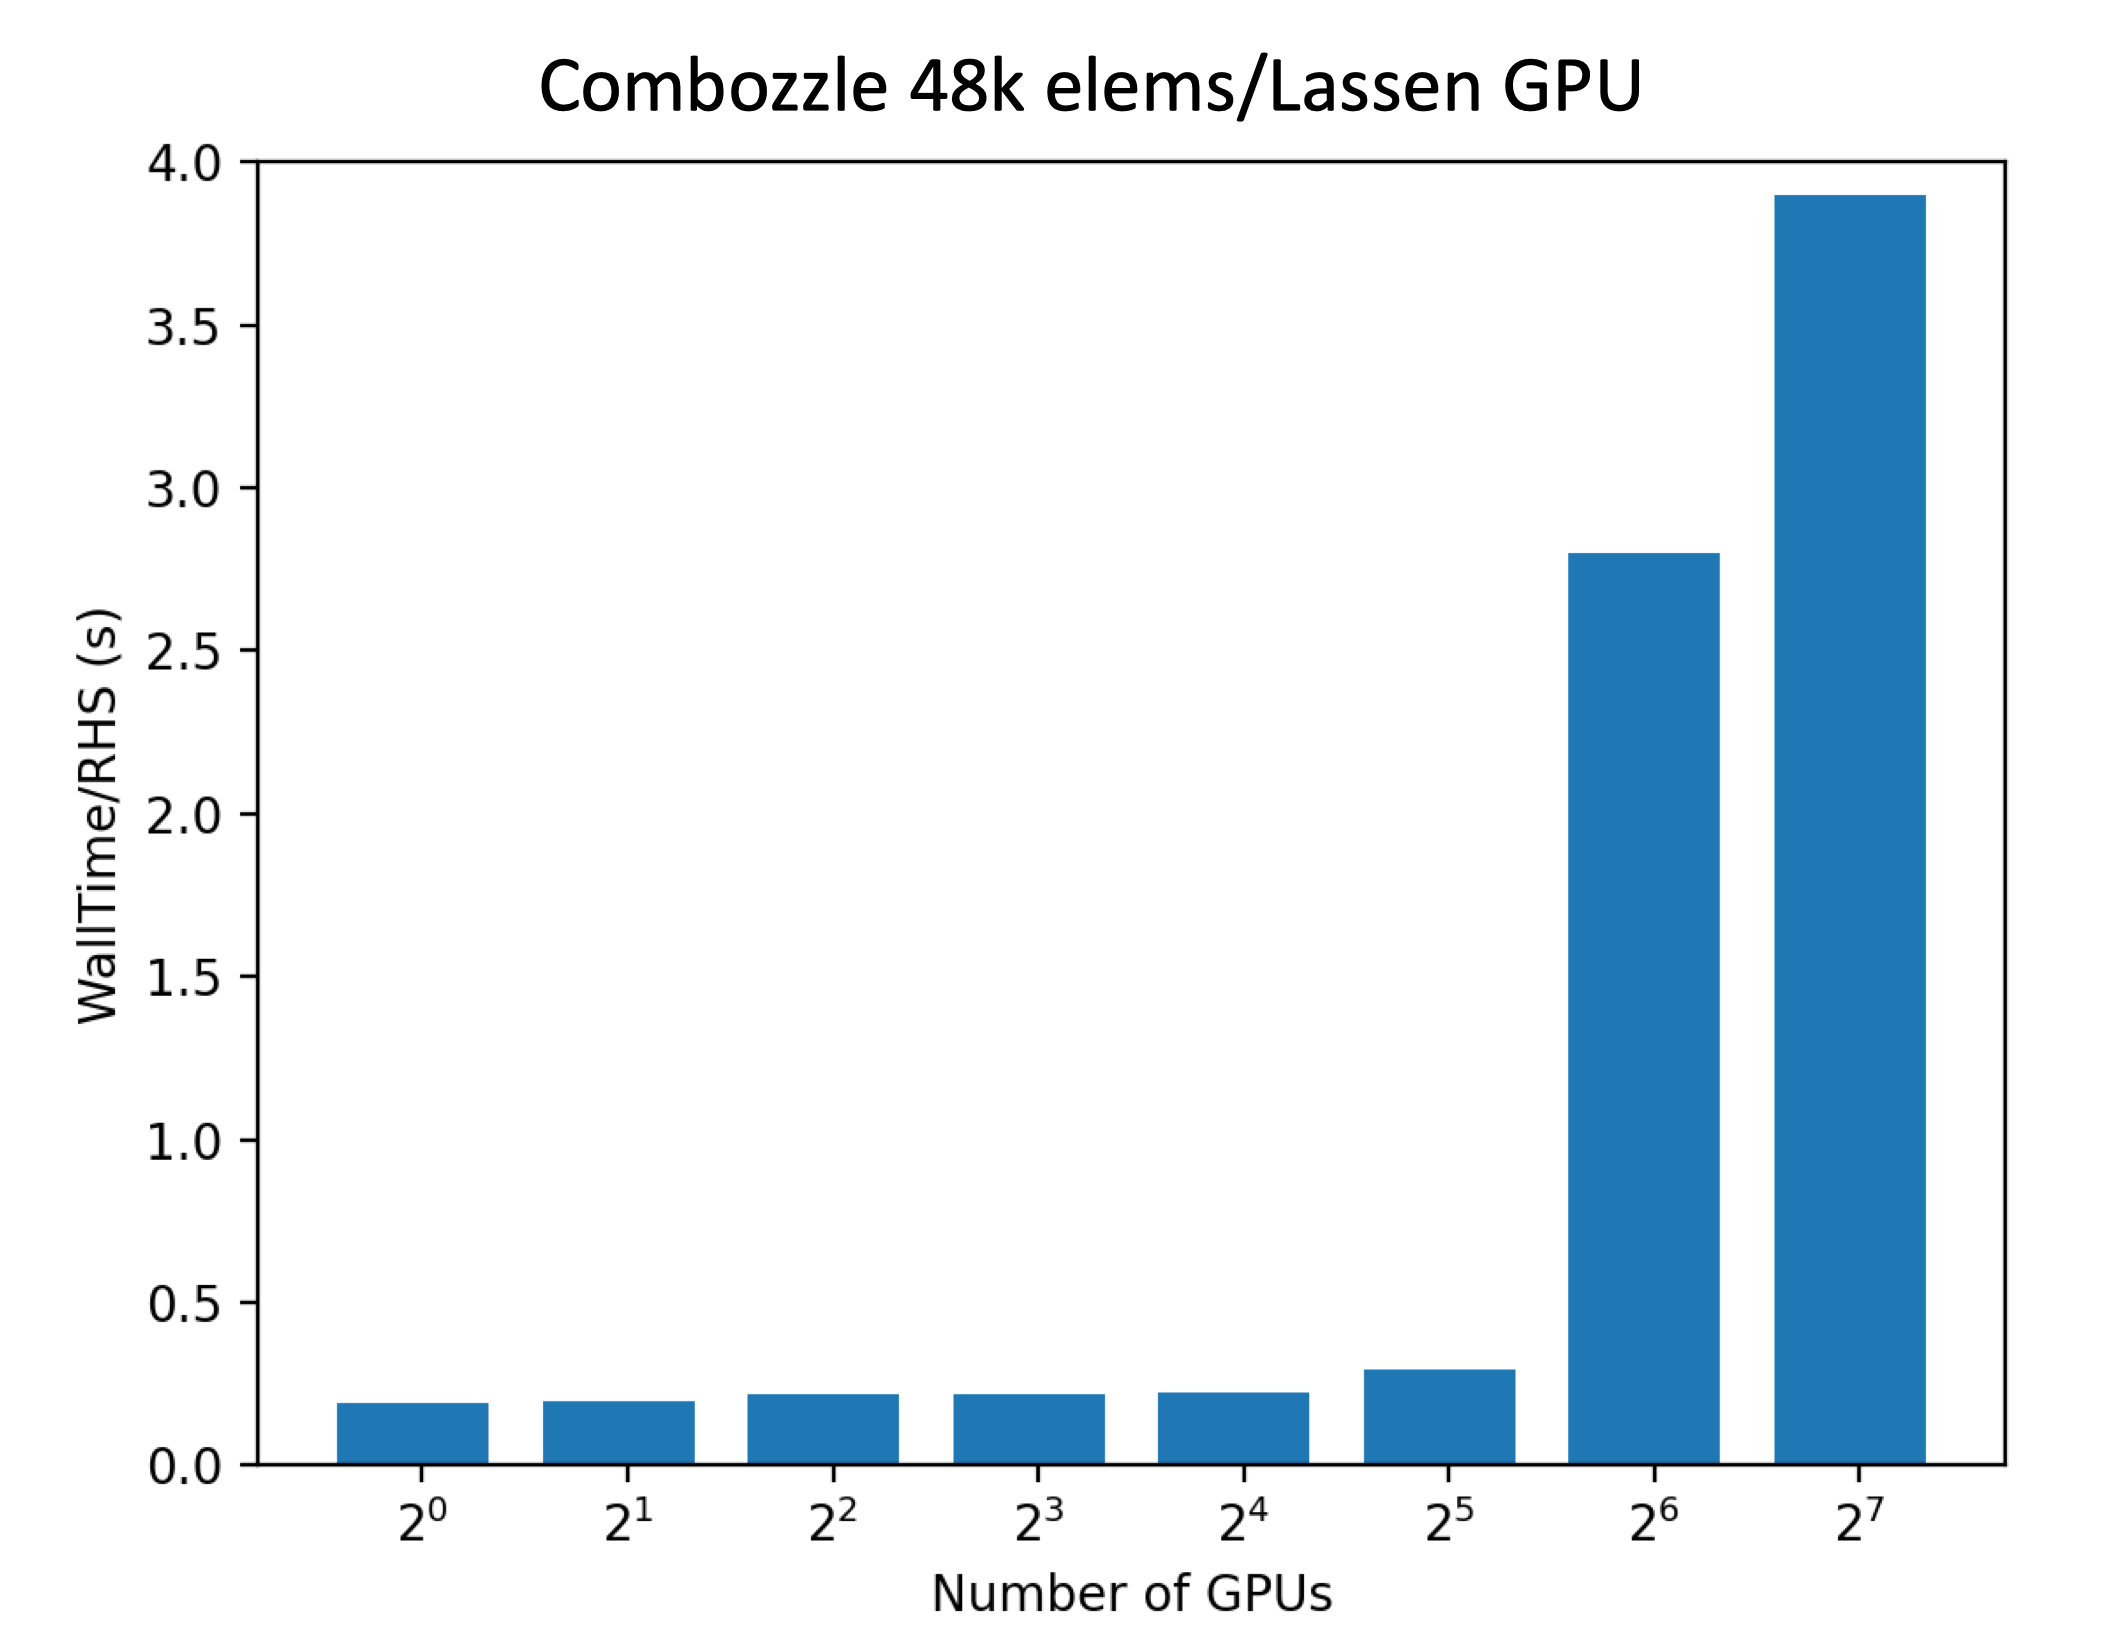
\includegraphics[width=.4\textwidth]{Figures/mtc/combozzle_weak_bad_partitioning.png}\hspace{30pt}
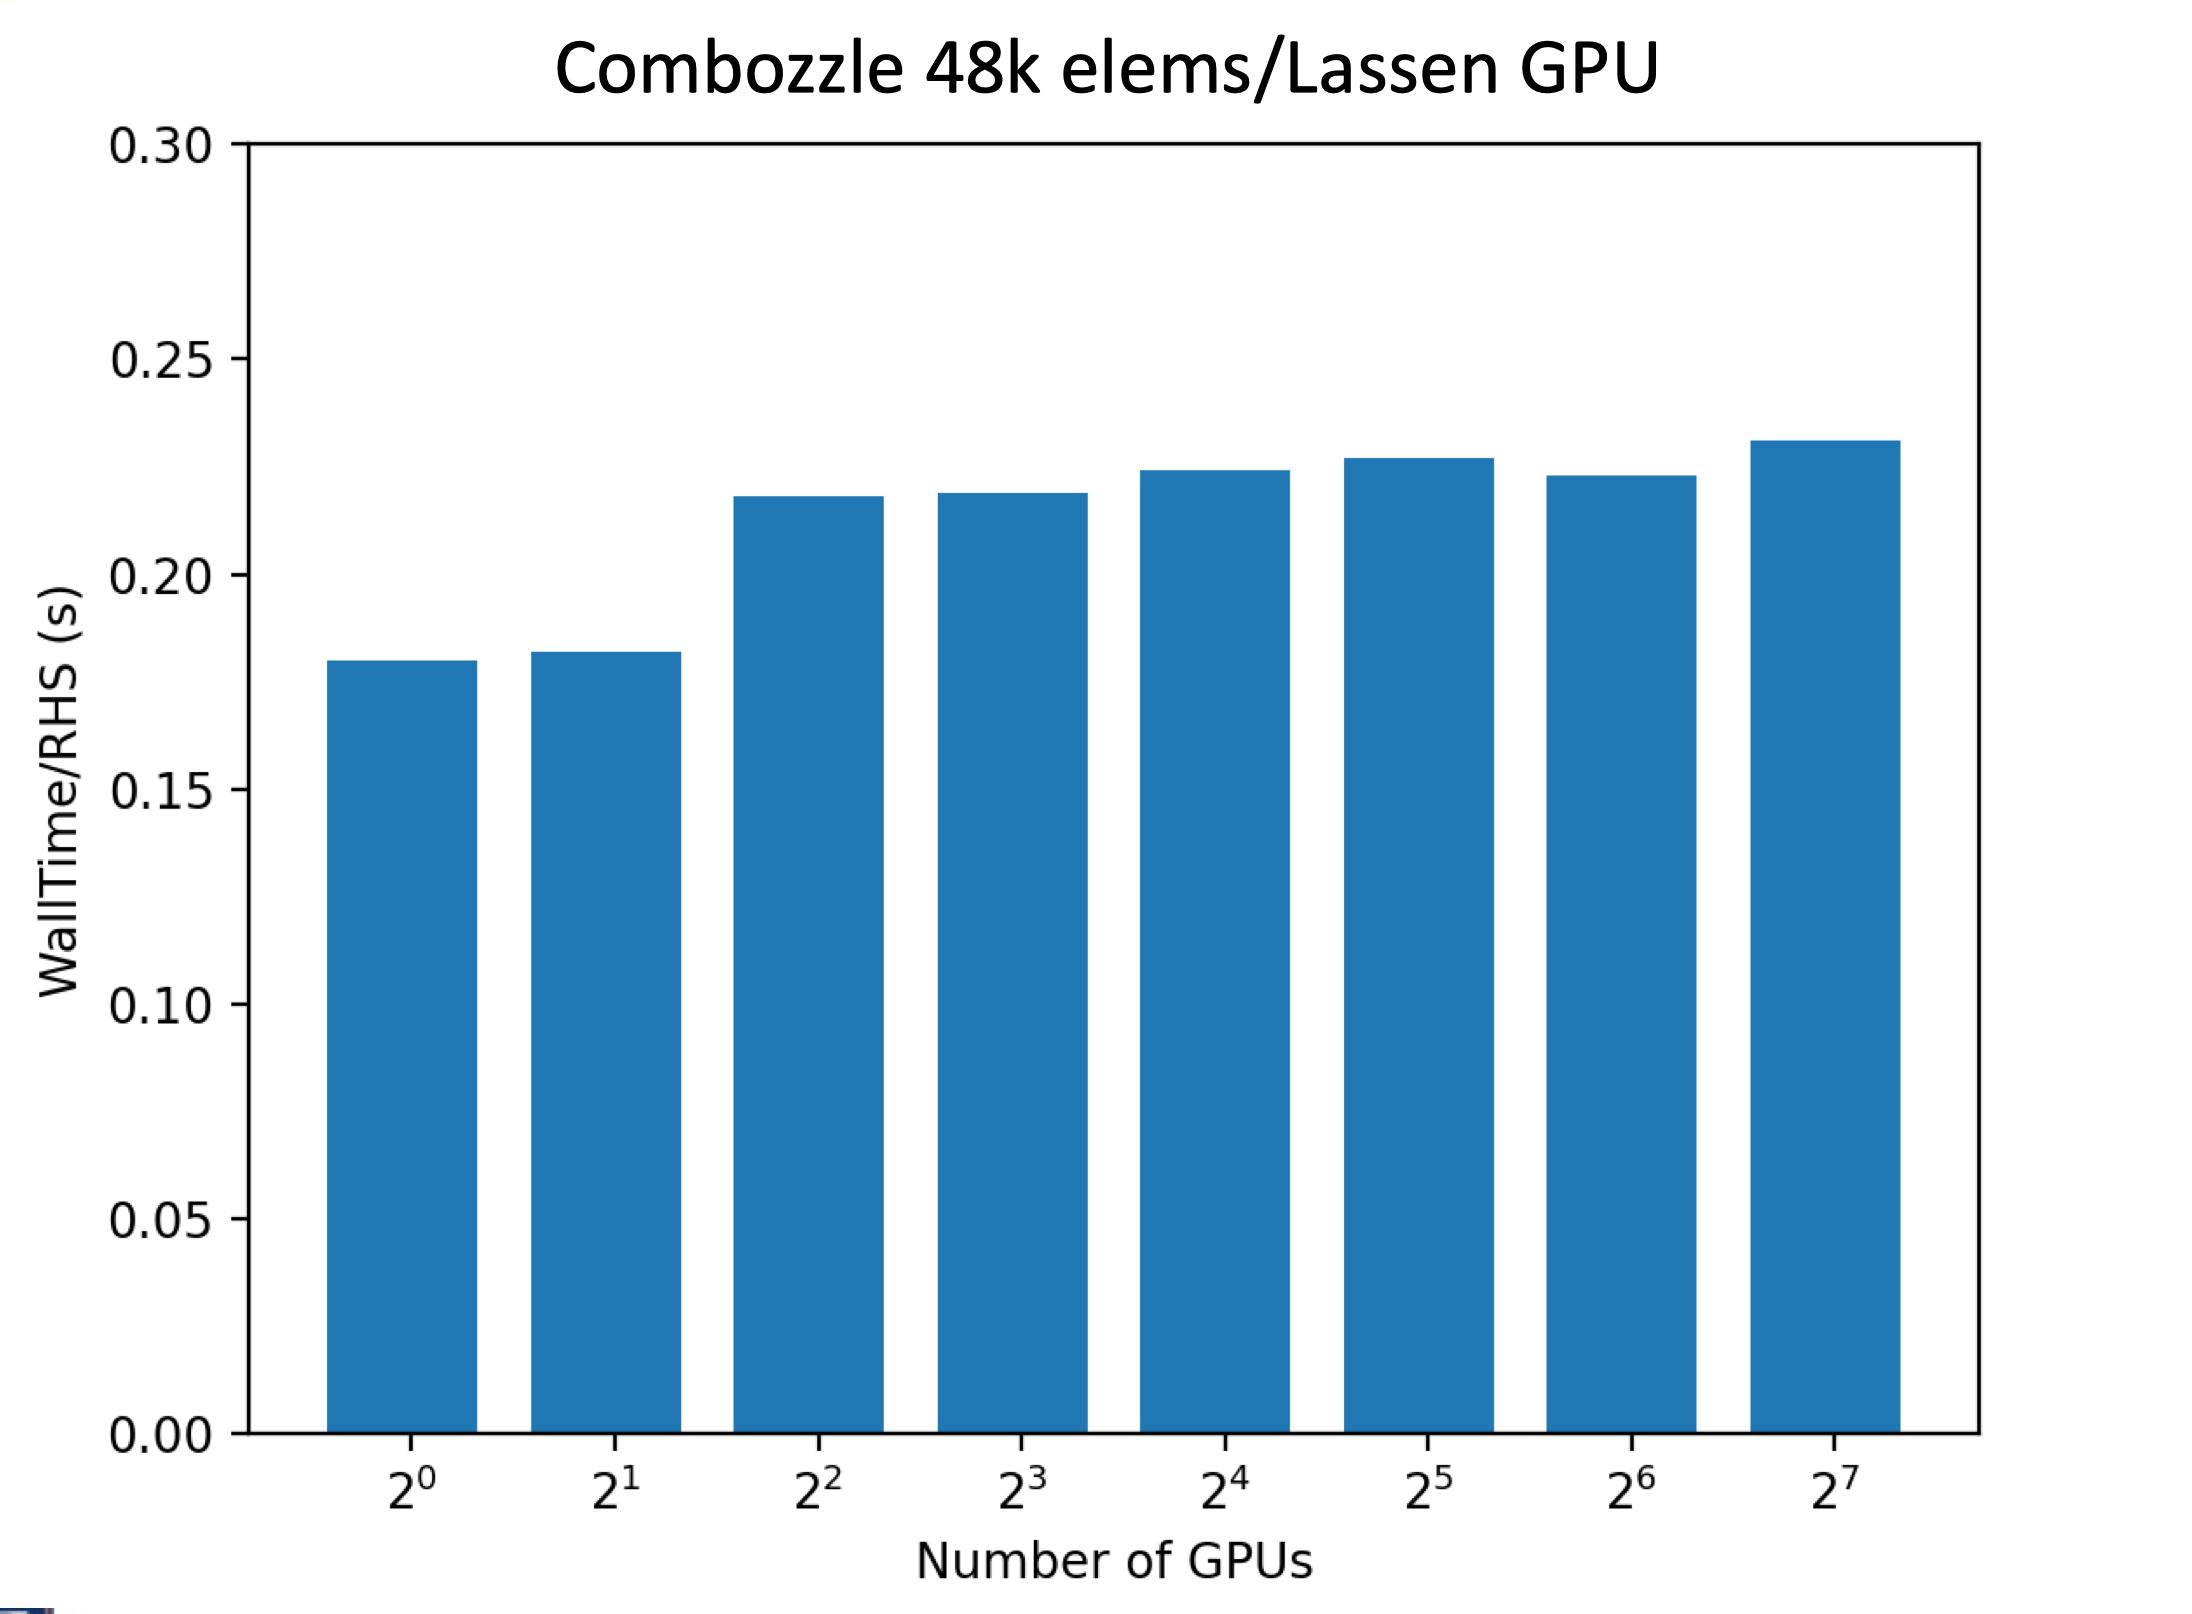
\includegraphics[width=.4\textwidth]{Figures/mtc/combozzle_weak_sliced_partitioning.png}
\end{minipage}
\end{frame}

\begin{frame}\frametitle{Performance}
\begin{minipage}[t][0.4\textheight][t]{\textwidth}
\begin{center}
New: prediction-enabling performance
\end{center}
\begin{multicols}{2}
\begin{itemize}
\item DAG Splat: DAG for each boundary
\item Limits weak scaling - DAG for each neighbor
\columnbreak
\item Mitigation: Metis $\to$ 1D decomp
\item Real fix: Function calls in the DAG \prj\tiny{Kaushik Kulkarni}
\end{itemize}
\end{multicols}
\end{minipage}\vfill
%\vspace{-100pt}
\begin{minipage}[t][0.4\textheight][t]{\textwidth}
\centering
%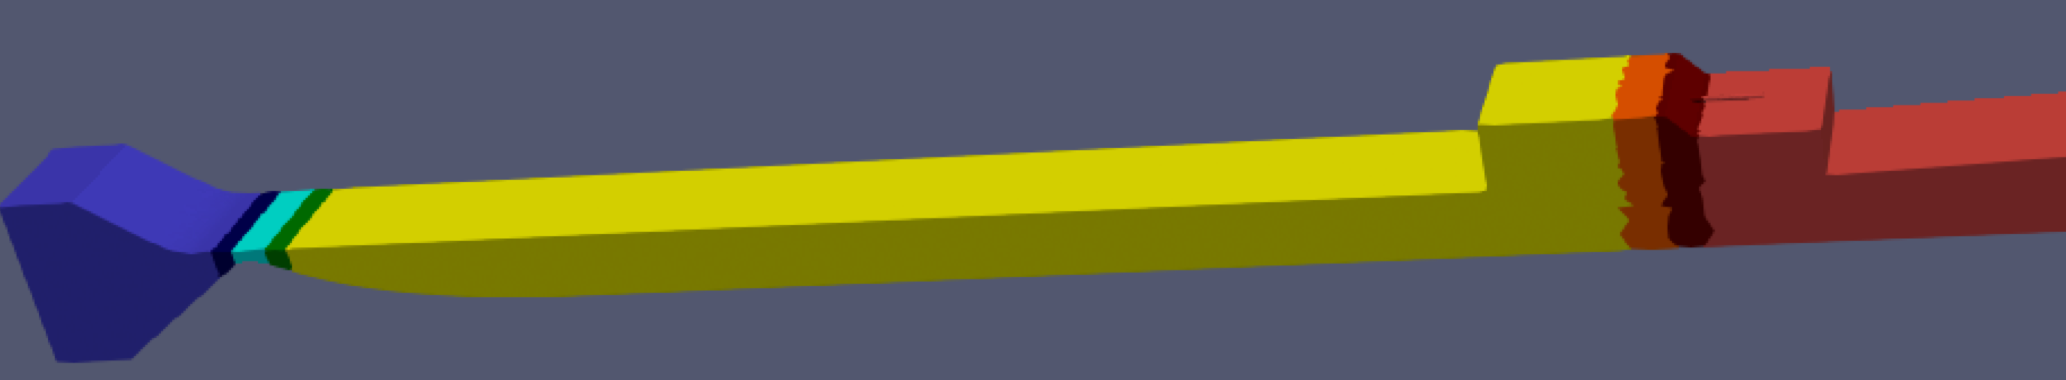
\includegraphics[width=.9\textwidth]{Figures/mtc/1dpart_bal.png}\\
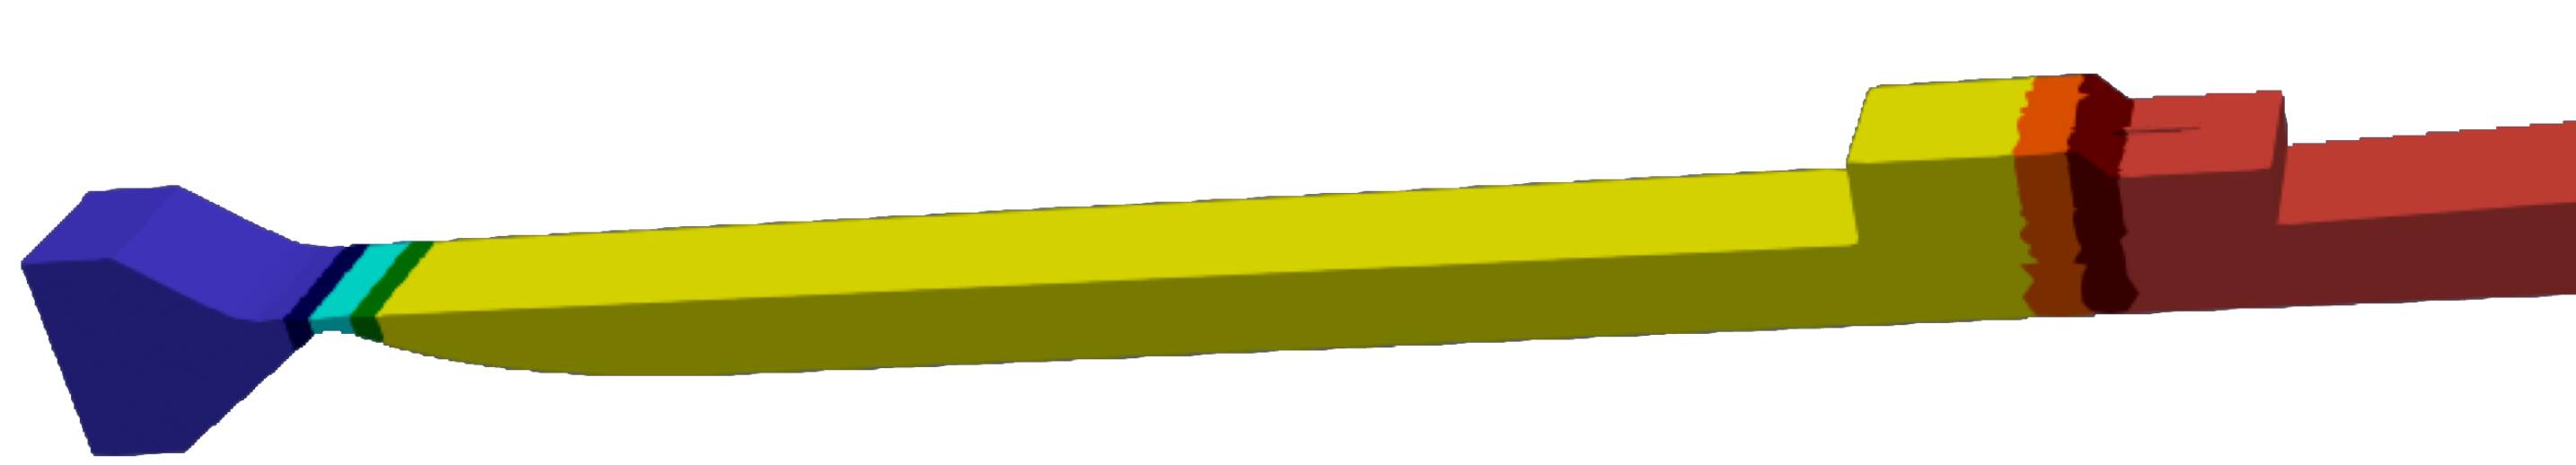
\includegraphics[width=.9\textwidth]{Figures/mtc/1dpartshiny.png}\\
%\vspace{-50pt}
\begin{center}
Y2 Domain Decomposition
\end{center}
\end{minipage}
\end{frame}

\begin{frame}\frametitle{Performance}
\begin{minipage}[t][0.4\textheight][t]{\textwidth}
\begin{center}
New: prediction-enabling performance
\end{center}
\begin{multicols}{2}
\begin{itemize}
\item DAG Splat: DAG for each boundary
\item Limits weak scaling - DAG for each neighbor
\columnbreak
\item Mitigation: Metis vs. 1D decomp
\item Real fix: Function calls in the DAG \prj\tiny{Kaushik Kulkarni}
\end{itemize}
\end{multicols}
\end{minipage}\vfill
\vspace{-20pt}
\begin{minipage}[t][0.4\textheight][t]{\textwidth}
\centering
%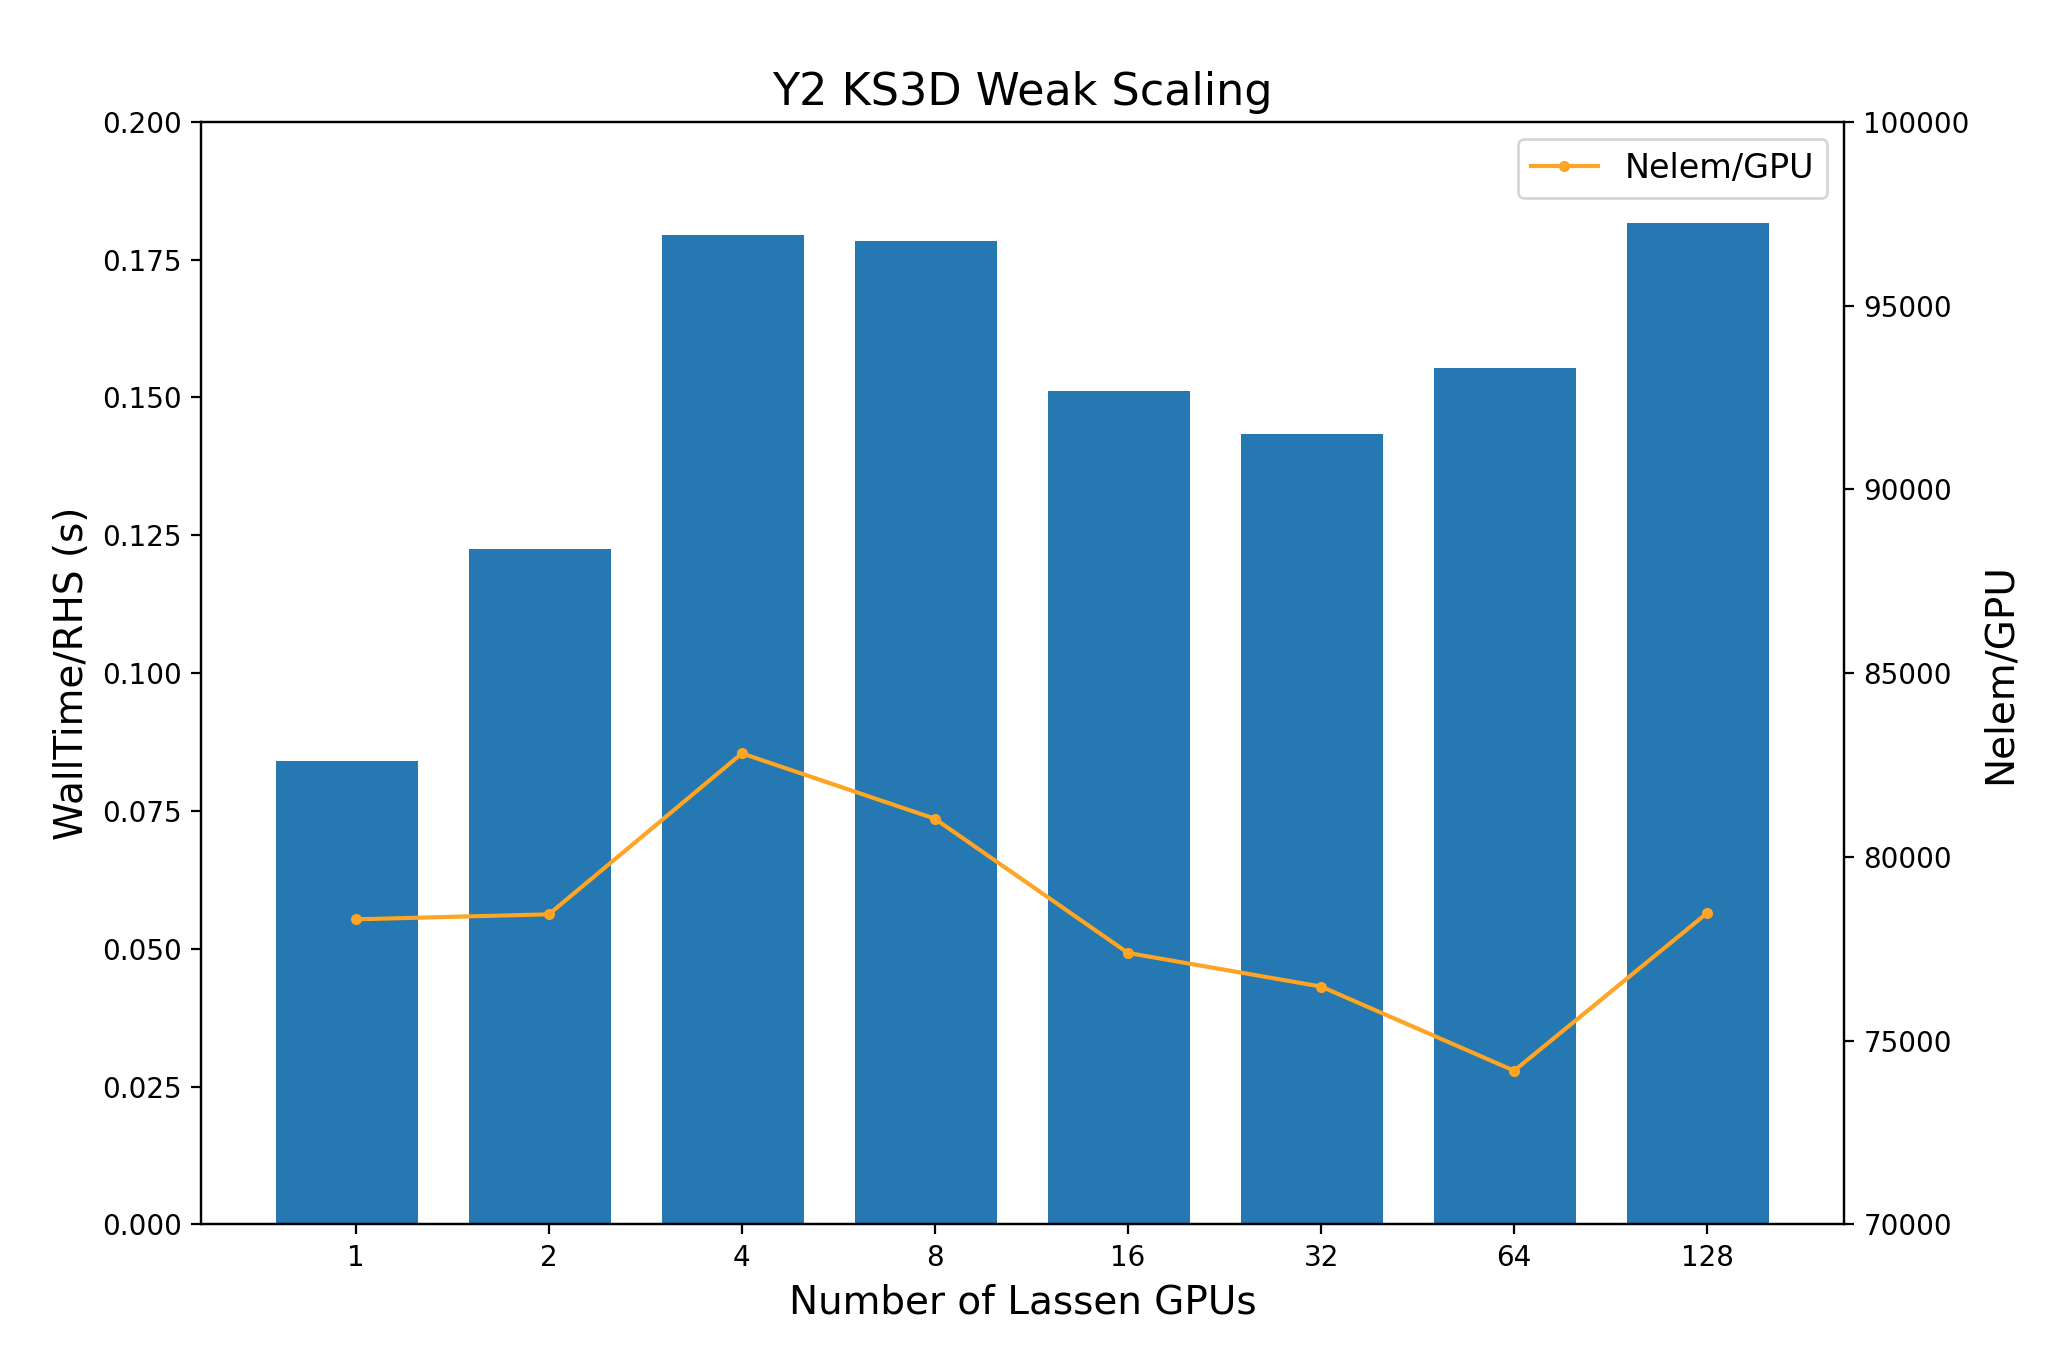
\includegraphics[width=.48\textwidth]{Figures/mtc/y2ks3d_weak.png}
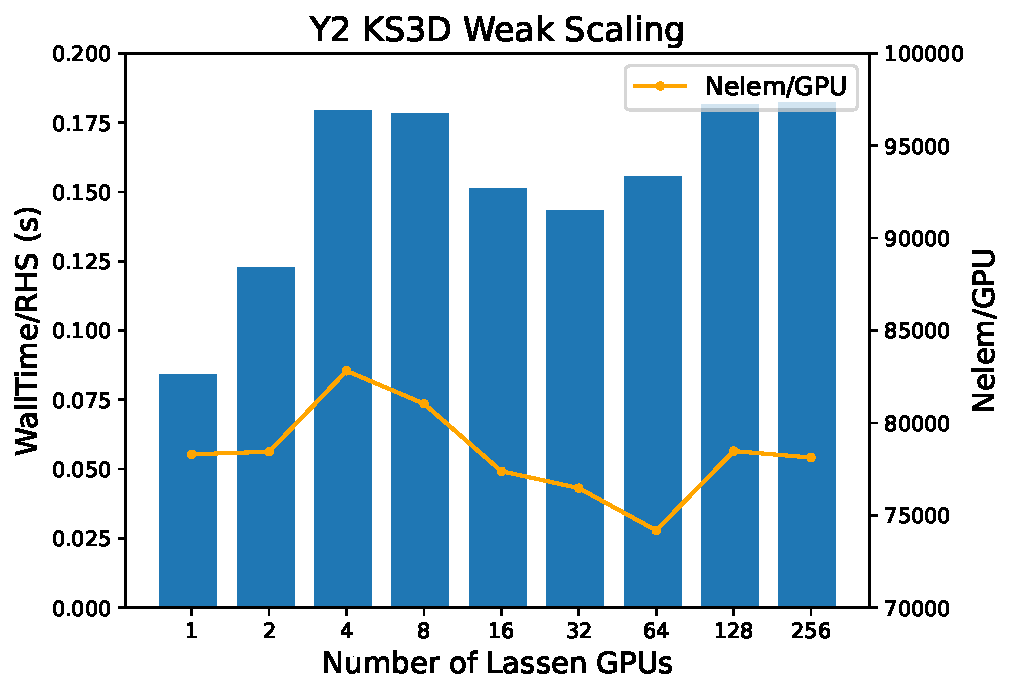
\includegraphics[width=.48\textwidth]{Figures/mtc/y2-prediction_weak_scaling.pdf}
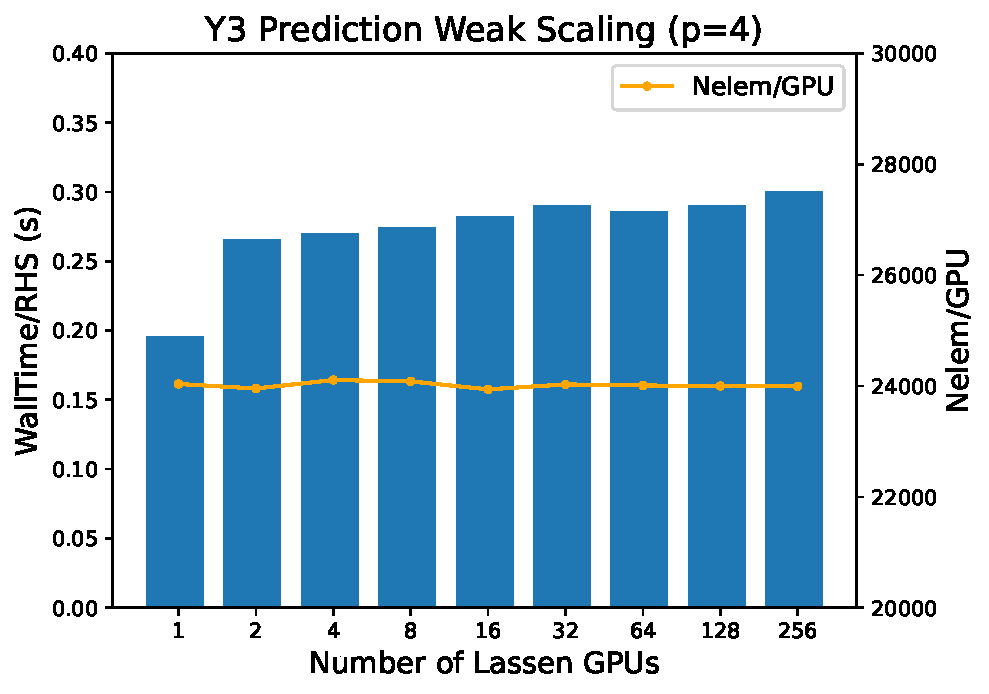
\includegraphics[width=.48\textwidth]{Figures/mtc/y3-prediction_weak_scaling.pdf}
\end{minipage}
\end{frame}

\begin{frame}\frametitle{Performance Monitoring on Lassen}
\begin{center}
https://github.com/illinois-ceesd/timing\\
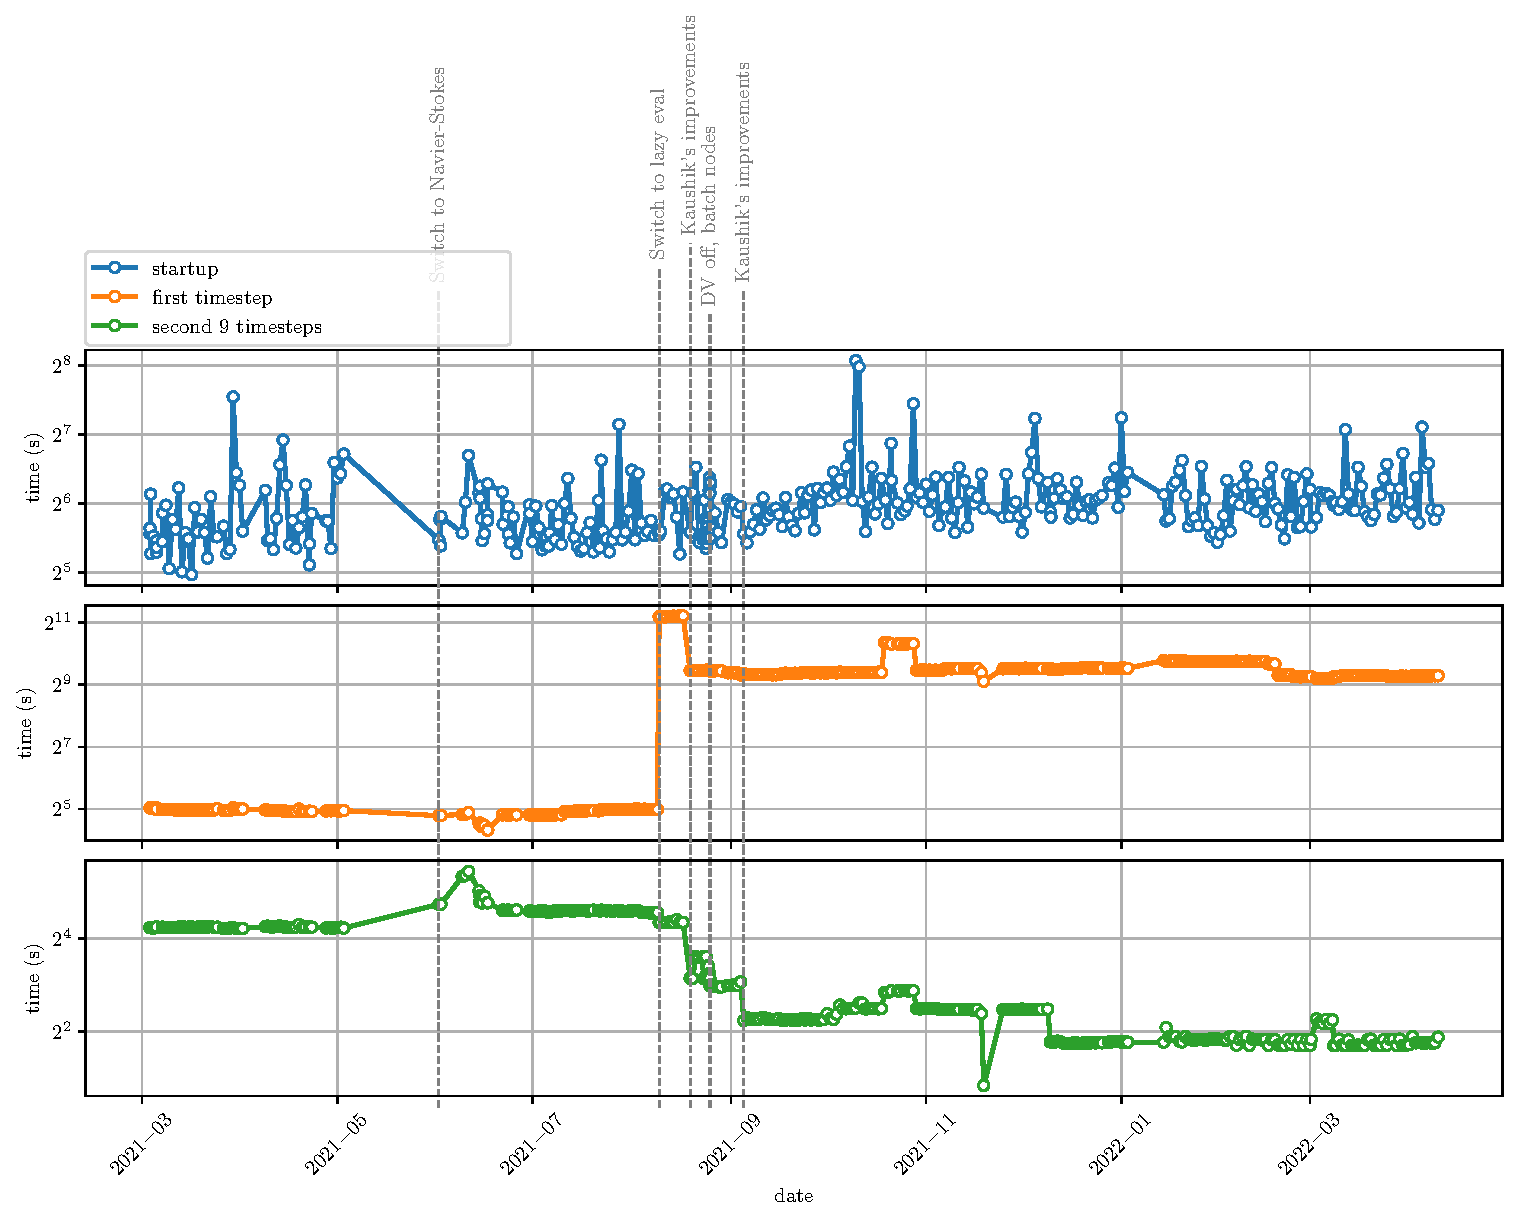
\includegraphics[width=.6\textwidth]{Figures/mtc/nozzle-lazy-full.pdf}
\end{center}
\end{frame}

\begin{frame}\frametitle{Performance Monitoring on Lassen}
\begin{minipage}[t][0.3\textheight][t]{\textwidth}
\begin{center}
https://github.com/illinois-ceesd/timing
\end{center}
\begin{multicols}{2}
\begin{itemize}
\item Data on key capabilities collected nightly
\item Intended to track performance vs. code/features
\item $\Delta$'s indicate change in performance
\columnbreak
\item New this cycle:
\begin{itemize}
\item Multi-case/comparitive plotting
\item Tracking parallel cases
\end{itemize}
\end{itemize}
\end{multicols}
\end{minipage}\vfill
\begin{center}
  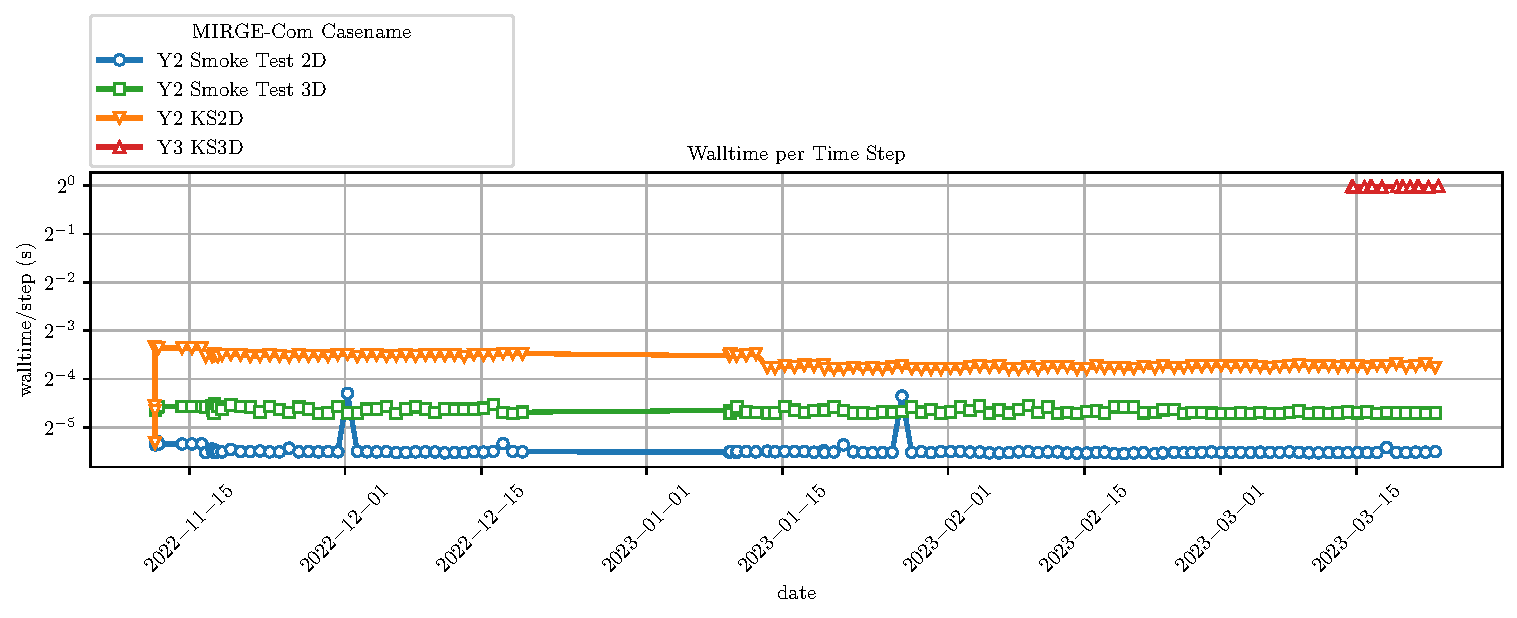
\includegraphics[width=.8\textwidth]{Figures/mtc/multicase_step.pdf}
\end{center}
\end{frame}

\begin{frame}\frametitle{Performance Monitoring on Lassen}
\begin{minipage}[t][0.3\textheight][t]{\textwidth}
\begin{center}
https://github.com/illinois-ceesd/timing
\end{center}
\begin{multicols}{2}
\begin{itemize}
\item Data on key capabilities collected nightly
\item Intended to track performance vs. code/features
\item $\Delta$'s indicate change in performance
\columnbreak
\item New this cycle:
\begin{itemize}
\item Multi-case/comparitive plotting
\item Tracking parallel cases
\end{itemize}
\end{itemize}
\end{multicols}
\end{minipage}\vfill
\begin{center}
  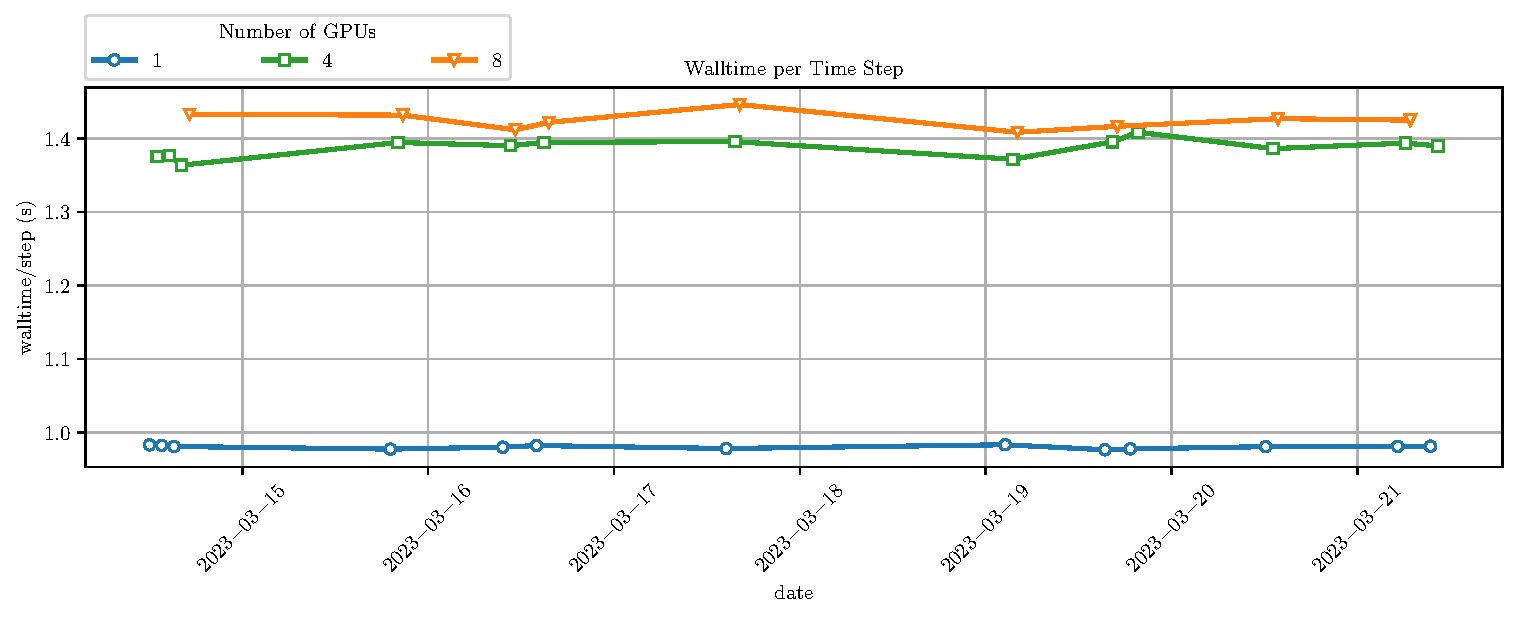
\includegraphics[width=.8\textwidth]{Figures/mtc/prediction-scaling-tracking.pdf}
\end{center}
\end{frame}

\begin{frame}\frametitle{Performance Monitoring on Lassen}
\begin{minipage}[t][0.3\textheight][t]{\textwidth}
\begin{center}
https://github.com/illinois-ceesd/timing
\end{center}
\begin{multicols}{2}
\begin{itemize}
\item Data on key capabilities collected nightly
\item Intended to track performance vs. code/features
\item $\Delta$'s indicate change in performance
\columnbreak
\item New this cycle:
\begin{itemize}
\item Multi-case/comparitive plotting
\item Tracking parallel cases
\end{itemize}
\end{itemize}
\end{multicols}
\end{minipage}\vfill
\begin{center}
  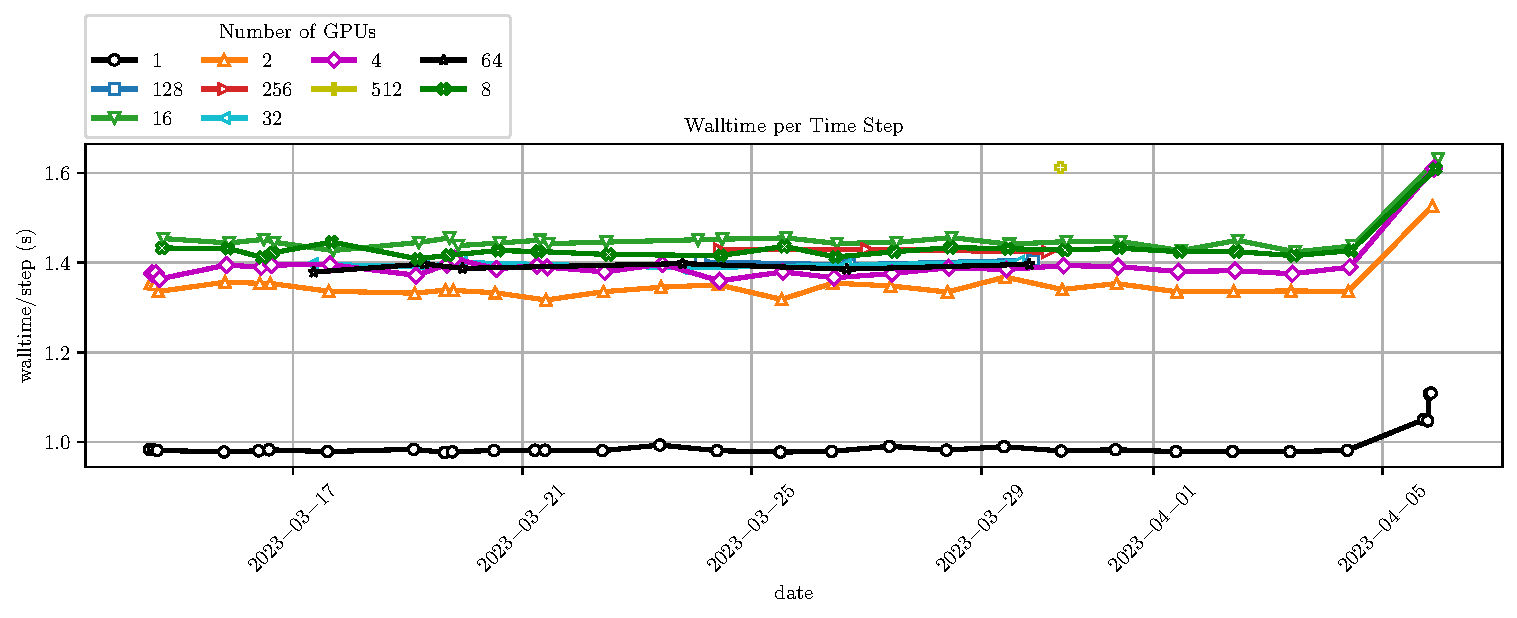
\includegraphics[width=.8\textwidth]{Figures/mtc/y3-prediction-parallel-20230405.pdf}
\end{center}
\end{frame}

\begin{frame}
    \centering
    \Large
    \textbf{Code Challenges}
\end{frame}

\begin{frame}\frametitle{M-to-N Restarts}
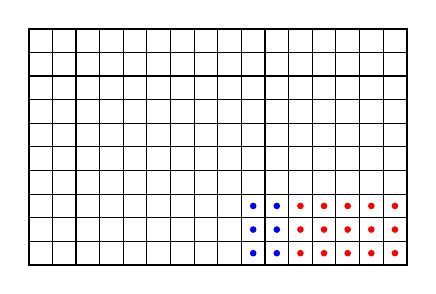
\begin{tikzpicture}[scale=0.3]
    % Grid
    \draw[step=1, thin, black] (0,0) grid (16,10);
    \draw[thick] (0,0) rectangle (16,10);
    
    % Red subregion
    \foreach \i in {11, 12, 13, 14, 15} {
        \foreach \j in {0, 1, 2} {
            \fill[red] (\i+0.5, \j+0.5) circle (4pt);
        }
    }
    
    % Blue subregion
    \foreach \i in {9, 10} {
        \foreach \j in {0, 1, 2} {
            \fill[blue] (\i+0.5, \j+0.5) circle (4pt);
        }
    }
\end{tikzpicture}
\end{frame}

\begin{frame}\frametitle{M-to-N Restarts}
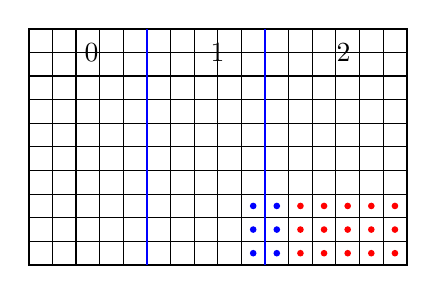
\begin{tikzpicture}[scale=0.3]
    % Grid
    \draw[step=1, thin, black] (0,0) grid (16,10);
    \draw[thick] (0,0) rectangle (16,10);
    
    % Red subregion
    \foreach \i in {11, 12, 13, 14, 15} {
        \foreach \j in {0, 1, 2} {
            \fill[red] (\i+0.5, \j+0.5) circle (4pt);
        }
    }
    
    % Blue subregion
    \foreach \i in {9, 10} {
        \foreach \j in {0, 1, 2} {
            \fill[blue] (\i+0.5, \j+0.5) circle (4pt);
        }
    }

    % Partition lines and labels for 3 partitions
    \draw[thick, blue] (5,0) -- (5,10);
    \draw[thick, blue] (10,0) -- (10,10);
    
    \node at (2.66,9) {0};
    \node at (7.99,9) {1};
    \node at (13.33,9) {2};
\end{tikzpicture}
\end{frame}

\begin{frame}\frametitle{M-to-N Restarts}
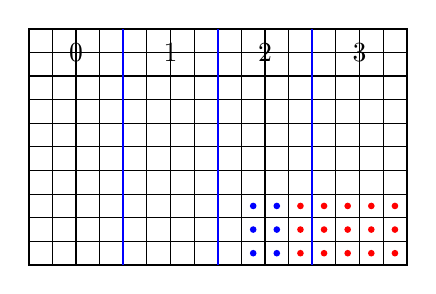
\begin{tikzpicture}[scale=0.3]
    % Grid
    \draw[step=1, thin, black] (0,0) grid (16,10);
    \draw[thick] (0,0) rectangle (16,10);
    
    % Red subregion
    \foreach \i in {11, 12, 13, 14, 15} {
        \foreach \j in {0, 1, 2} {
            \fill[red] (\i+0.5, \j+0.5) circle (4pt);
        }
    }
    
    % Blue subregion
    \foreach \i in {9, 10} {
        \foreach \j in {0, 1, 2} {
            \fill[blue] (\i+0.5, \j+0.5) circle (4pt);
        }
    }

    % Partition lines and labels
    \draw[thick, blue] (4,0) -- (4,10);
    \draw[thick, blue] (8,0) -- (8,10);
    \draw[thick, blue] (12,0) -- (12,10);

    \node at (2,9) {0};
    \node at (6,9) {1};
    \node at (10,9) {2};
    \node at (14,9) {3};
\end{tikzpicture}
\end{frame}


\begin{frame}\frametitle{M-to-N Restarts}
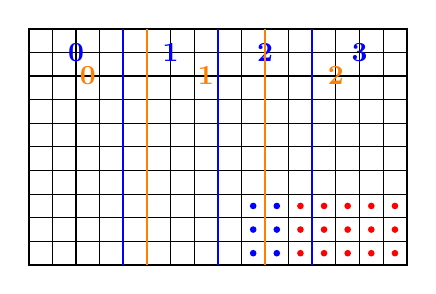
\begin{tikzpicture}[scale=0.3]
    % Grid
    \draw[step=1, thin, black] (0,0) grid (16,10);
    \draw[thick] (0,0) rectangle (16,10);
    
    % Red subregion
    \foreach \i in {11, 12, 13, 14, 15} {
        \foreach \j in {0, 1, 2} {
            \fill[red] (\i+0.5, \j+0.5) circle (4pt);
        }
    }
    
    % Blue subregion
    \foreach \i in {9, 10} {
        \foreach \j in {0, 1, 2} {
            \fill[blue] (\i+0.5, \j+0.5) circle (4pt);
        }
    }

    % Partition lines and labels for 4 partitions (in blue)
    \draw[thick, blue] (4,0) -- (4,10);
    \draw[thick, blue] (8,0) -- (8,10);
    \draw[thick, blue] (12,0) -- (12,10);
    
    \node[font=\bfseries, blue] at (2,9) {0};
    \node[font=\bfseries, blue] at (6,9) {1};
    \node[font=\bfseries, blue] at (10,9) {2};
    \node[font=\bfseries, blue] at (14,9) {3};

    % Partition lines for 3 partitions (in orange)
    \draw[thick, orange] (5,0) -- (5,10);
    \draw[thick, orange] (10,0) -- (10,10);
    
    \node[font=\bfseries, orange] at (2.5,8) {0};
    \node[font=\bfseries, orange] at (7.5,8) {1};
    \node[font=\bfseries, orange] at (13,8) {2};
\end{tikzpicture}
\end{frame}

\begin{frame}
\frametitle{M-to-N Restart}
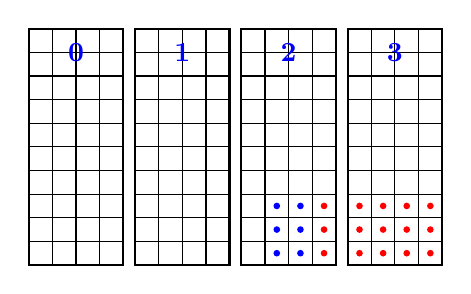
\begin{tikzpicture}[scale=0.3]

    % Partition 0
    \draw[step=1, thin, black] (0,0) grid (4,10);
    \draw[thick] (0,0) rectangle (4,10);
    \node[font=\bfseries, blue] at (2,9) {0};
    
    % Partition 1
    \begin{scope}[xshift=4.5cm]
        \draw[step=1, thin, black] (0,0) grid (4,10);
        \draw[thick] (0,0) rectangle (4,10);
        \node[font=\bfseries, blue] at (2,9) {1};
    \end{scope}
    
    % Partition 2 with blue and red subregions
    \begin{scope}[xshift=9cm]
        \draw[step=1, thin, black] (0,0) grid (4,10);
        \draw[thick] (0,0) rectangle (4,10);
        \foreach \j in {0, 1, 2} {
            \fill[blue] (1.5, \j+0.5) circle (4pt);
            \fill[blue] (2.5, \j+0.5) circle (4pt);
            \fill[red] (3.5, \j+0.5) circle (4pt);
        }
        \node[font=\bfseries, blue] at (2,9) {2};
    \end{scope}
    
    % Partition 3 with red subregion
    \begin{scope}[xshift=13.5cm]
        \draw[step=1, thin, black] (0,0) grid (4,10);
        \draw[thick] (0,0) rectangle (4,10);
        \foreach \j in {0, 1, 2} {
            \fill[red] (0.5, \j+0.5) circle (4pt);
            \fill[red] (1.5, \j+0.5) circle (4pt);
            \fill[red] (2.5, \j+0.5) circle (4pt);
            \fill[red] (3.5, \j+0.5) circle (4pt);  % added this line for the last column of red dots in partition 3
        }
        \node[font=\bfseries, blue] at (2,9) {3};
    \end{scope}
\end{tikzpicture}
\end{frame}

\begin{frame}
\frametitle{M-to-N Restart}
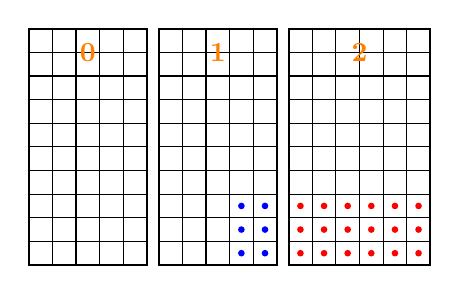
\begin{tikzpicture}[scale=0.3]

    % Partition 0
    \draw[step=1, thin, black] (0,0) grid (5,10);
    \draw[thick] (0,0) rectangle (5,10);
    \node[font=\bfseries, orange] at (2.5,9) {0};
    
    % Partition 1 with blue subregion
    \begin{scope}[xshift=5.5cm]
        \draw[step=1, thin, black] (0,0) grid (5,10);
        \draw[thick] (0,0) rectangle (5,10);
        \foreach \j in {0, 1, 2} {
            \fill[blue] (3.5, \j+0.5) circle (4pt);
            \fill[blue] (4.5, \j+0.5) circle (4pt);
        }
        \node[font=\bfseries, orange] at (2.5,9) {1};
    \end{scope}
    
    % Partition 2 with red subregion
    \begin{scope}[xshift=11cm]
        \draw[step=1, thin, black] (0,0) grid (6,10);
        \draw[thick] (0,0) rectangle (6,10);
        \foreach \j in {0, 1, 2} {
            \fill[red] (0.5, \j+0.5) circle (4pt);
            \fill[red] (1.5, \j+0.5) circle (4pt);
            \fill[red] (2.5, \j+0.5) circle (4pt);
            \fill[red] (3.5, \j+0.5) circle (4pt);
            \fill[red] (4.5, \j+0.5) circle (4pt);
            \fill[red] (5.5, \j+0.5) circle (4pt);
        }
        \node[font=\bfseries, orange] at (3,9) {2};
    \end{scope}
\end{tikzpicture}
\end{frame}

%\begin{frame}
%\frametitle{Grid without Border on Cutout}
%\begin{tikzpicture}[scale=0.3]
%
%    % Draw only the visible cells
%    \foreach \i in {0,1,2,3} {
%        \foreach \j in {3,4,...,9} {
%            \draw (\i,\j) rectangle (\i+1,\j+1);
%        }
%    }
%    \draw (0,0) rectangle (1,3);
%    \draw (0,0) rectangle (1,1);
%    \draw (0,1) rectangle (1,2);
%    \draw (0,2) rectangle (1,3);
%
%    % Adjusted border
%    \draw[thick] (0,0) -- (1,0) -- (1,3) -- (4,3) -- (4,10) -- (0,10) -- cycle;
%
%\end{tikzpicture}
%\end{frame}

\begin{frame}
\frametitle{M-to-N Restart}
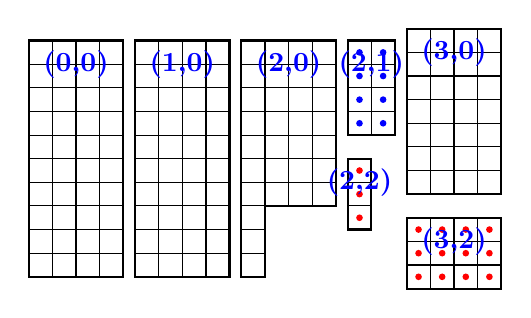
\begin{tikzpicture}[scale=0.3]

    % Partition (0,0)
    \draw[step=1, thin, black] (0,0) grid (4,10);
    \draw[thick] (0,0) rectangle (4,10);
    \node[font=\bfseries, blue] at (2,9) {(0,0)};

    % Partition (1,0)
    \begin{scope}[xshift=4.5cm]
        \draw[step=1, thin, black] (0,0) grid (4,10);
        \draw[thick] (0,0) rectangle (4,10);
        \node[font=\bfseries, blue] at (2,9) {(1,0)};
    \end{scope}

    % Partition (2,0) with the correct shape and border
    \begin{scope}[xshift=9cm]
        \foreach \i in {0,1,2,3} {
            \foreach \j in {3,4,...,9} {
                \draw (\i,\j) rectangle (\i+1,\j+1);
            }
        }
        \draw (0,0) rectangle (1,3);
        \draw (0,0) rectangle (1,1);
        \draw (0,1) rectangle (1,2);
        \draw (0,2) rectangle (1,3);
        \draw[thick] (0,0) -- (1,0) -- (1,3) -- (4,3) -- (4,10) -- (0,10) -- cycle;
        \node[font=\bfseries, blue] at (2,9) {(2,0)};
    \end{scope}

    % Partition (2,1) with blue subregion, adjusted position
    \begin{scope}[xshift=13.5cm, yshift=6cm]
        \draw[step=1, thin, black] (0,0) grid (2,4);
        \draw[thick] (0,0) rectangle (2,4);
        \foreach \j in {0,1,2,3} {
            \fill[blue] (0.5, \j+0.5) circle (4pt);
            \fill[blue] (1.5, \j+0.5) circle (4pt);
        }
        \node[font=\bfseries, blue] at (1,3) {(2,1)};
    \end{scope}

    % Partition (2,2) with red subregion, adjusted position
    \begin{scope}[xshift=13.5cm, yshift=2cm]
        \draw[step=1, thin, black] (0,0) grid (1,3);
        \draw[thick] (0,0) rectangle (1,3);
        \foreach \j in {0,1,2} {
            \fill[red] (0.5, \j+0.5) circle (4pt);
        }
        \node[font=\bfseries, blue] at (0.5,2) {(2,2)};
    \end{scope}

    % Partition (3,0), adjusted position and dimensions
    \begin{scope}[xshift=16cm, yshift=3.5cm]
        \draw[step=1, thin, black] (0,0) grid (4,7);
        \draw[thick] (0,0) rectangle (4,7);
        \node[font=\bfseries, blue] at (2,6) {(3,0)};
    \end{scope}

    % Partition (3,2) with red subregion, adjusted position
    \begin{scope}[xshift=16cm, yshift=-0.5cm]
        \draw[step=1, thin, black] (0,0) grid (4,3);
        \draw[thick] (0,0) rectangle (4,3);
        \foreach \j in {0,1,2} {
            \fill[red] (0.5, \j+0.5) circle (4pt);
            \fill[red] (1.5, \j+0.5) circle (4pt);
            \fill[red] (2.5, \j+0.5) circle (4pt);
            \fill[red] (3.5, \j+0.5) circle (4pt);
        }
        \node[font=\bfseries, blue] at (2,2) {(3,2)};
    \end{scope}

\end{tikzpicture}
\end{frame}

\begin{frame}
\frametitle{M-to-N Restart}
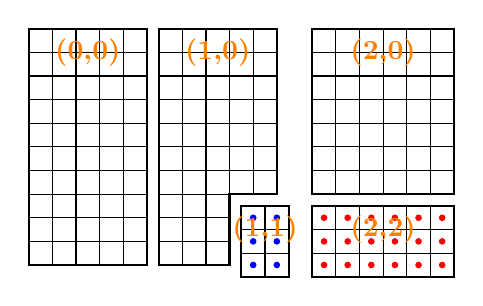
\begin{tikzpicture}[scale=0.3]

    % Partition (0,0)
    \draw[step=1, thin, black] (0,0) grid (5,10);
    \draw[thick] (0,0) rectangle (5,10);
    \node[font=\bfseries, orange] at (2.5,9) {(0,0)};

    % Partition (1,0) with the correct shape, border, and panhandle grid
    \begin{scope}[xshift=5.5cm]
        \foreach \i in {0,1,2,3,4} {
            \foreach \j in {3,4,...,9} {
                \draw (\i,\j) rectangle (\i+1,\j+1);
            }
        }
        \foreach \i in {0,1,2} {
            \foreach \j in {0,1,2} {
                \draw (\i,\j) rectangle (\i+1,\j+1);
            }
        }
        \draw[thick] (0,0) -- (3,0) -- (3,3) -- (5,3) -- (5,10) -- (0,10) -- cycle;
        \node[font=\bfseries, orange] at (2.5,9) {(1,0)};
    \end{scope}

    % Partition (1,1) with blue subregion, further adjusted position
    \begin{scope}[xshift=9cm, yshift=-0.5cm]
        \draw[step=1, thin, black] (0,0) grid (2,3);
        \draw[thick] (0,0) rectangle (2,3);
        \foreach \j in {0,1,2} {
            \fill[blue] (0.5, \j+0.5) circle (4pt);
            \fill[blue] (1.5, \j+0.5) circle (4pt);
        }
        \node[font=\bfseries, orange] at (1,2) {(1,1)};
    \end{scope}

    % Partition (2,0)
    \begin{scope}[xshift=12cm, yshift=3cm]
        \draw[step=1, thin, black] (0,0) grid (6,7);
        \draw[thick] (0,0) rectangle (6,7);
        \node[font=\bfseries, orange] at (3,6) {(2,0)};
    \end{scope}

    % Partition (2,2) with red subregion
    \begin{scope}[xshift=12cm, yshift=-0.5cm]
        \draw[step=1, thin, black] (0,0) grid (6,3);
        \draw[thick] (0,0) rectangle (6,3);
        \foreach \j in {0,1,2} {
            \fill[red] (0.5, \j+0.5) circle (4pt);
            \fill[red] (1.5, \j+0.5) circle (4pt);
            \fill[red] (2.5, \j+0.5) circle (4pt);
            \fill[red] (3.5, \j+0.5) circle (4pt);
            \fill[red] (4.5, \j+0.5) circle (4pt);
            \fill[red] (5.5, \j+0.5) circle (4pt);
        }
        \node[font=\bfseries, orange] at (3,2) {(2,2)};
    \end{scope}

\end{tikzpicture}
\end{frame}

\begin{frame}
\frametitle{M-to-N Restart}

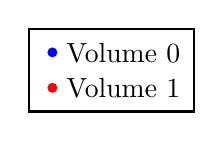
\begin{tikzpicture}[scale=0.3]
    % ... [rest of your existing TikZ picture]

    % Legend Box
    \begin{scope}[xshift=20cm, yshift=8cm]
        \draw[thick] (-1,0.5) rectangle (6,-3); % Adjusted the top border of the box
        
        \fill[blue] (0,-0.5) circle (6pt); % Blue dot
        \node[align=left] at (3,-0.5) {Volume 0}; % Moved the label to the right
        
        \fill[red] (0,-2) circle (6pt);  % Red dot
        \node[align=left] at (3,-2) {Volume 1}; % Moved the label to the right
    \end{scope}
\end{tikzpicture}
\end{frame}

\begin{frame}\frametitle{M-to-N Restarts}
\end{frame}

\begin{frame}
    \centering
    \Large
    \textbf{Wrapping Up \& Looking Ahead}
\end{frame}


\begin{frame}\frametitle{Summary and Next Steps}
\begin{itemize}
\item \mirgecom{} has Y3 prediction-supporting performance (poised to deliver more)
\item Understanding \mirgecom{} performance is the next major focus
\end{itemize}
\begin{center}
Next steps
\end{center}
\begin{multicols}{2}
\begin{itemize}
\item Understanding and improving performance:
\begin{itemize}
\item Instrumentation (Mem \& Tags) \prj{\tiny}{Kaushik Kulkarni, M.~Diener}
\item Code-to-kernel correspondence improvements: \prj{\tiny}{07c, M.~Diener}
\item Auto-tuning \prj{\tiny}{Nick Christensen}
\item Node-aware communicators \prj{\tiny}{Shelby Lockhart}
\item \sout{DAG Splat} \prj{\tiny}{Kaushik Kulkarni}
\item Performance model
\end{itemize}
\item Upcoming enhancements:
\begin{itemize}
\item Workflow: \textit{Parsl} \prj{\tiny}{D.~Friedel}
\item Testing: Mixtures and BCs: Moser MMS
\item Entropy-Stable DG \prj{\tiny}{Zurui Wang}
\item Hexahedral elements \prj{\tiny}{Addison Alvey-Blanco}
\item M-to-N restart (HDF5)
\end{itemize}
\end{itemize}
%\columnbreak
%\end{multicols}
%\vspace{-20pt}
%\begin{center}
%  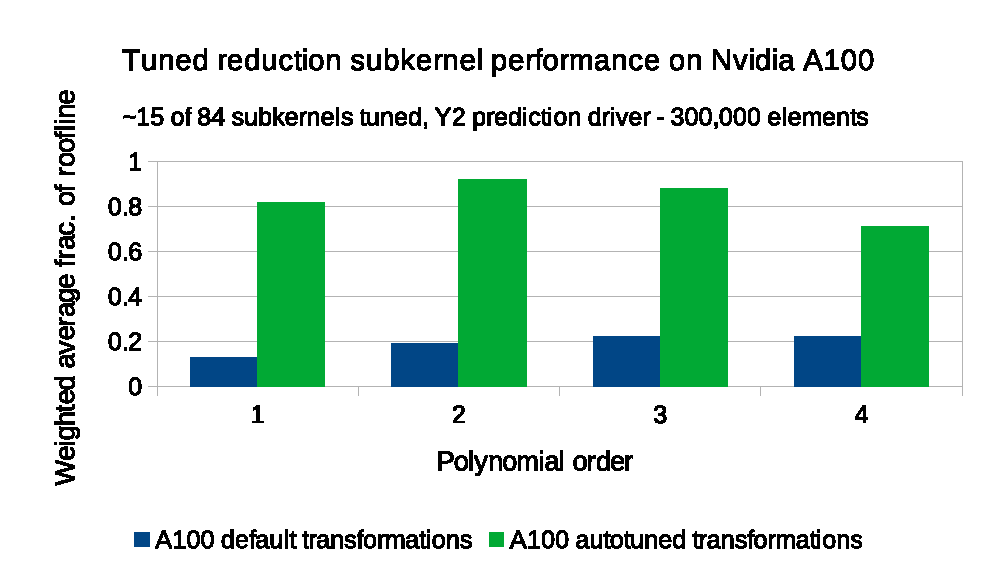
\includegraphics[width=.48\textwidth]{Figures/mtc/Nvidia-A100-performance.eps}
%  \prj{\tiny}{Nick Christensen}
%\end{center}
\end{multicols}
\end{frame}

% - PLANS CHANGE
%\begin{frame}\frametitle{Developments for Y3 Prediction}
%\begin{center}
%Y3 Driver\\
%https://github.com/illinois-ceesd/drivers\_y3-prediction
%\end{center}
%\begin{multicols}{2}
%\begin{itemize}
%\item Kitchen sink (KS) feature set
%  \begin{itemize}
%  \item Coupled CNS + Wall/heat
%  \item Ethylene mixture, reaction sources, species limiting, power-law transport
%  \item Wall degradation, oxygen diffusion, reactive/porous mat.
%  \item Artificial physical viscosity, and sponge
%  \item OFF: Mixture transport, spectral filtering on RHS
 % \end{itemize}
%\item Meshes: 2D/3D updated geom, 2 test sects., shallower cavity
%\item Sims: 3D coupled (6M,p=4 256 GPUs), and smaller
%\item Scalability scripting and inputs (@add-scalability)
%\end{itemize}
%\end{multicols}
%\end{frame}

%\begin{frame}\frametitle{Path to Y3 Prediction}
%\begin{multicols}{2}
%\begin{itemize}
%\item Physics and modeling: Radiation \& Phenolics (mild gap)
%\item Numerics and discretization
%  \begin{itemize}
%  \item Mesh modifications (upstream injector, possible refinement)
%  \item Maybe (gaps suspected):
%    \begin{itemize}
%    \item Higher order mesh + filtering (likely!)
%    \item New AV
%    % \item Slope limiters
%    \item Multi-order meshes/volumes
%    \item ESDG? \prj{\tiny}{Zirui Wang}
%    \item Stop gap: High viscosity, maybe reduced physics
%    \end{itemize}
%  \end{itemize}
%\columnbreak
%\item Performance - closing gaps
%  \begin{itemize}
%  \item Cost per step (inert, comb): (.5, 1.4)s
%  \item Sim time: 1ms inert, 6e-4 w/comb
%  \item Estimated DT: .5ns
%  \item 12d inert, 19d comb
%  \item Any improvements welcomed
%  \end{itemize}
%\end{itemize}
%\end{multicols}
%\end{frame}

%\begin{frame}\frametitle{Path to Y3 Prediction}
%\begin{center}
%\item Preparing for prediction runs
%\end{center}
%\begin{multicols}{2}
%\begin{itemize}
%\item 3M(ish) 3D p=3 elems 
%\item Potentially serious issues: Shock/boundary, fluid/material
%\item Investigating higher order, with filtering, high visc
%\item Many scoping, physics-targeted, and debugging runs
%\end{itemize}
%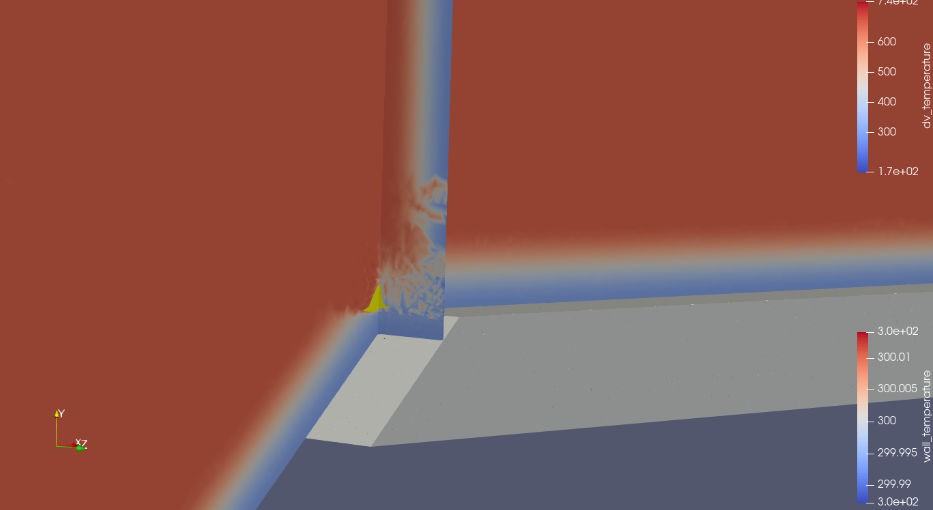
\includegraphics[width=.3\textwidth]{Figures/mtc/hot_edge.png}
%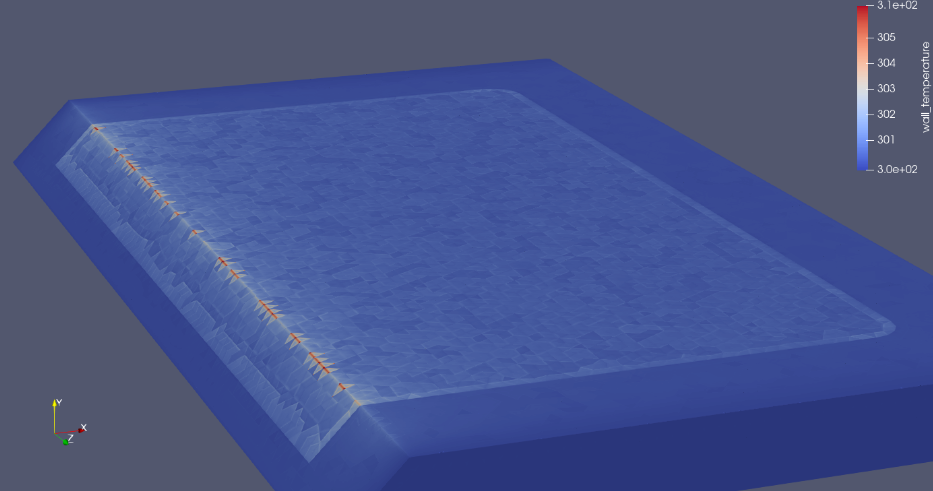
\includegraphics[width=.4\textwidth]{Figures/mtc/3d_yellow_cells.png}
%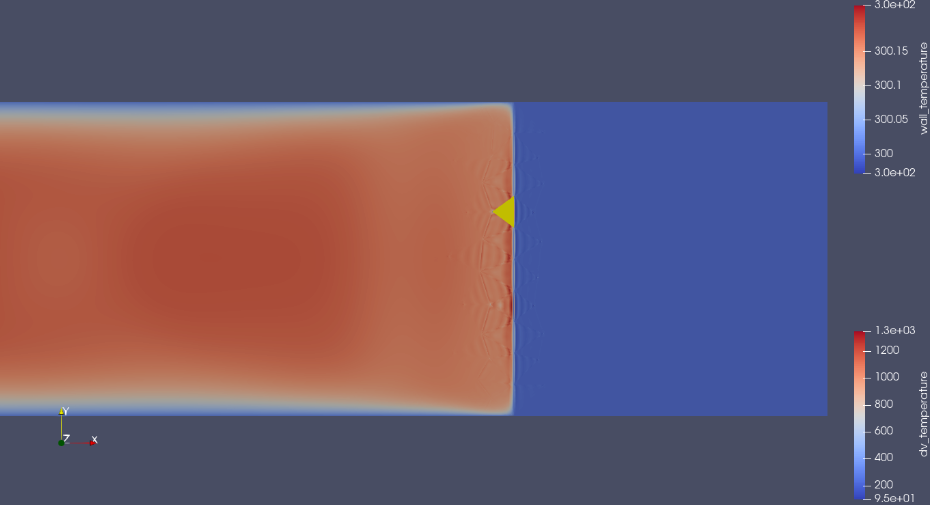
\includegraphics[width=.4\textwidth]{Figures/mtc/2d_yellow_cells.png}
%\end{multicols}
%\end{frame}

%\begin{frame}\frametitle{Path to Y3 Prediction}
%\begin{multicols}{2}
%\begin{itemize}
%\item Some pain points
%  \begin{itemize}
%  \item Transfinite or ultra fine mesh to stabilize fluid boundary
    % \begin{itemize}
    % \item Increases complexity of meshing by a lot
    % \item Increases number of elements
    % \item Hex support desired, might help
    % \end{itemize}
%  \item Lack confidence in correctness of model implementation
    % \begin{itemize}
    % \item Problem with numerics, or defect?
    % \item More extensive testing!
    % \item More experience/intuition about the numerics
    % \item ESDG?, FV?
    % \end{itemize}
%  \item Small problem performance is a drag
    % \begin{itemize}
    % \item 20m compile (this is fine, not fine)
    % \item DAG splat elim, faster compile
    % \end{itemize}
%  \item Makes lots of big files
    % \begin{itemize}
    % \item PARSL
    % \item Viz Driver
    % \end{itemize}
%  \item Development and testing viscosity
%  \item Long queues on available platforms
%  \item Cannot change size of run to adapt to resources
%  \end{itemize}
%\end{itemize}
%\end{multicols}
%\end{frame}


%\begin{frame}\frametitle{Near-term Development Outlook}
%\begin{multicols}{2}
%\begin{itemize}
%\item Now
%  \begin{itemize}
%  \item Understanding performance (why is it hard?)
%    \begin{itemize}
%    \item Code $\leftrightarrow$ Kernel \prj{\tiny}{M.~Diener}
%    \item Performance model
%    \item Kernel rooflines \prj{\tiny}{Nick Christensen}
%    \item Feature-specific
%    \end{itemize}
%  \item Evaluate Tioga
%  \item Boundary verif (MMS)
%  \item PARSL for testing \prj{\tiny}{D.~Friedel}
%  \end{itemize}
%\end{itemize}
%\columnbreak
%\begin{itemize}
%\item For prediction: (4mo horizon)
%  \begin{itemize}
%  \item Radiation \& phenolics \prj{\tiny}{T.~Ricciardi, M.~Smith}
%  \item \sout{DAG splat} \prj{\tiny}{Kaushik Kulkarni}
%  \item Mechanism parameterization for UQ
%  \item PARSL for UQ \prj{\tiny}{D.~Friedel}
%  \item Stabilizing prediction runs \prj{\tiny}{M.~Anderson}
%    \begin{itemize}
%    \item ESDG \prj{\tiny}{Zirui Wang}
%    \item Mixed-order
%    \item Quad/Hex support \prj{\tiny}{Addison Alvey-Blanco}
%    \item Curvlinear elements
%    \end{itemize}
%  \end{itemize}
%\end{itemize}
%\end{multicols}
%\end{frame}

%\begin{frame}\frametitle{Nice to have any time}
%\begin{multicols}{2}
%\begin{itemize}
%\item Reducing prediction pain (important):
%  \begin{itemize}
%  \item Reduce technical debt (merges)
%  \item Driver unification
%  \item Help with mesh generation
%  \item Visualization driver
%  \item PARSL for queue management
%  \item M-to-N restart
 % \end{itemize}
%%\item Potentially high-impact performance improvements
%  \begin{itemize}
%  \item Kernel Autotuning \prj{\tiny}{Nick Christensen}
%  \item Node-aware communication \prj{\tiny}{Shelby Lockhart}
%  \item DAG/compile time improvements \prj{\tiny}{Kaushik Kulkarni, M.~Diener}
%  \item Instrumentation (Mem \& Tags) \prj{\tiny}{Kaushik Kulkarni, M.~Diener}
%  \end{itemize}
%\item Future sims
%  \begin{itemize}
%  \item Mesh motion (interface regression)
%  \item Wall degradation
%  \item Turbulence modeling
%  \end{itemize}
%\end{itemize}
%\end{multicols}
%\end{frame}



%======================================================================
\begin{frame}\frametitle{}

\vspace*{0.2in}

\begin{center}


\includegraphics[width=0.35\textwidth]{../ceesd-logo-2.pdf}

\vspace*{0.35in}
\cPI{\huge Questions?}

\vspace*{0.5in}
\begin{minipage}{0.6\textwidth}
This material is based in part upon work supported by the Department of Energy, National Nuclear Security Administration, under Award Number DE-NA0003963. 
\end{minipage}



\end{center}


\end{frame}
%======================================================================


\end{document}
